\section{Experiments}
\subsection{Experimental setup}
Whole implementation was written in Python language using
PyTorch, Numpy, Pillow and Torchvision libraries
and is available at
\url{https://github.com/kamieen03/mgr}.
Implementation
of B-spline GCNNs is based on original Tensorflow version from
\cite{bekkers2019}.

Implemented models were trained and tested on CIFAR10 \cite{cifar},
CIFAR100 \cite{cifar} and STL10 \cite{stl10} datasets.
For STL10 only the labeled part of training set was used.

All implemented models are based on ResNet18 architecture \cite{resnet}.
Every network starts with initial convolution, normalization, activation
function and pooling layer. After that either $6$ (in CIFAR models)
or $8$ (in STL10 models) residual bottlenecks are
placed. Bottlenecks come in pairs, that is bottleneck no. $2k$ and no. $2k+1$
always have the same number of channels. We use list notation to denote size of
network, for example [$\mathit{n1}$; $\mathit{n2}$; $\mathit{n3}$]
is CIFAR model with $2$ bottlenecks with $n1$ channels, $2$ bottlenecks with
$n2$ channels and $2$ bottlenecks with $n3$ channels placed consecutively.
Every network ends with
fully-connected layer.

Overall there are 3 types of models:
\begin{itemize}
    \item \textbf{PlainResNet} is regular ResNet as described in \cite{resnet}.
    \item In \textbf{BsplineResNet} usual convolutional layers are replaced by
        B-spline group convolutional layers and the first convolution is replaced
        by lift operation. Network is parametrized by group $G$ it's supposed to be
        equivariant to and size of B-spline basis -- $N$ in equation
        \ref{eq:bsplines}. Model name is determined by $G$
    \item \textbf{BResNet} resemble Plain models, but standard normalization is
        replaced by mean normalization, so that the first couple layers are
        equivariant to change in brightness. The exact number of equivariant
        layers is parameter. In \textit{BrightnessEq} model all layers before
        final fully-connected layer are equivariant. In \textit{InBk} networks,
        a single $CBW$ layer is placed in the $k$th Bottleneck with all earlier
        Bottlenecks equivariant.
\end{itemize}
Plain and Bspline models can additionally have $\mathit{CBW}$ or $\mathit{GBW}$
layer at the very beginning of the network. In such case `\textit{+InCBW0}' or
`\textit{+InGBW0}' is added to their names. All architectures are detailed in
table \ref{tab:models_stl} and \ref{tab:models_cifar}. Particular layer sizes of
models in each table were selected in such a way to assure all of them have
roughly the same number of parameters. TODO- ile

\begin{table}[h!]
\centering
\begin{adjustbox}{center}
\begin{tabular}{c|c|c|>{\centering\arraybackslash}m{4em}|
    >{\centering\arraybackslash}m{7em}|>{\centering\arraybackslash}m{4em}}
 \hline
 \hline
 Model type & Model name & Numbers of channels & Initial invariant layer & Equivariance group &
 B-spline basis size \\
 \hline
 \hline
 \multirow{3}{7em}{PlainResNet} & Plain & [80; 160; 256; 256] & --- & --- & --- \\
     & Plain+InCBW0 & [80; 160; 256; 256] & CBW & --- & --- \\
     & Plain+InGBW0 & [80; 160; 256; 256] & GBW & --- & --- \\
 \hline
 \hline

 \multirow{10}{7em}{BsplineResNet} & RotEq & [32; 64; 64; 64] & --- & SO(2) & 12 \\
     & RotEq+InCBW0 & [32; 64; 64; 64] & CBW & SO(2) & 12 \\
     & RotEq+InGBW0 & [32; 64; 64; 64] & GBW & SO(2) & 12 \\
     & ScaleEq & [48; 64; 100; 128] & --- & Scale group & 5 \\
     & ScaleEq+InCBW0 & [48; 64; 100; 128] & CBW & Scale group & 5 \\
     & ScaleEq+InGBW0 & [48; 64; 100; 128] & GBW & Scale group & 5 \\
     & SchearEq & [48; 64; 100; 128] & --- & Schear group & 5 \\
     & SchearEq+InCBW0 & [48; 64; 100; 128] & CBW & Schear group & 5 \\
     & SchearEq+InGBW0 & [48; 64; 100; 128] & GBW & Schear group & 5 \\
     & GammmaEq & [48; 64; 100; 128] & --- & Gamma group & 5 \\
 \hline
 \hline

 \multirow{4}{7em}{BResNet} & BrightnessEq & [80; 160; 256; 256] & --- & --- & --- \\
     & InB1 & [80; 160; 256; 256] & --- & --- & --- \\
     & InB2 & [80; 160; 256; 256] & --- & --- & --- \\
     & InB3 & [80; 160; 256; 256] & --- & --- & --- \\
 \hline
 \hline
\end{tabular}
\end{adjustbox}
\caption{STL10 models}
\label{tab:models_stl}
\end{table}



\begin{table}[h!]
\centering
\begin{adjustbox}{center}
\begin{tabular}{c|c|c|>{\centering\arraybackslash}m{4em}|
    >{\centering\arraybackslash}m{7em}|>{\centering\arraybackslash}m{4em}}
 \hline
 \hline
 Model type & Model name & Numbers of channels & Initial invariant layer & Equivariance group &
 B-spline basis size \\
 \hline
 \hline
 \multirow{3}{7em}{PlainResNet} & Plain & [80; 160; 256] & --- & --- & --- \\
     & Plain+InCBW0 & [80; 160; 256] & CBW & --- & --- \\
     & Plain+InGBW0 & [80; 160; 256] & GBW & --- & --- \\
 \hline
 \hline

 \multirow{10}{7em}{BsplineResNet} & RotEq & [32; 48; 64] & --- & SO(2) & 12 \\
     & RotEq+InCBW0 & [32; 48; 64] & CBW & SO(2) & 12 \\
     & RotEq+InGBW0 & [32; 48; 64] & GBW & SO(2) & 12 \\
     & ScaleEq & [64; 96; 128] & --- & Scale group & 3 \\
     & ScaleEq+InCBW0 & [64; 96; 128] & CBW & Scale group & 3 \\
     & ScaleEq+InGBW0 & [64; 96; 128] & GBW & Scale group & 3 \\
     & SchearEq & [48; 72; 108] & --- & Schear group & 5 \\
     & SchearEq+InCBW0 & [48; 72; 108] & CBW & Schear group & 5 \\
     & SchearEq+InGBW0 & [48; 72; 108] & GBW & Schear group & 5 \\
     & GammmaEq & [48; 72; 108] & --- & Gamma group & 5 \\
 \hline
 \hline

 \multirow{4}{7em}{BResNet} & BrightnessEq & [80; 160; 256] & --- & --- & --- \\
     & InB1 & [80; 160; 256] & --- & --- & --- \\
     & InB2 & [80; 160; 256] & --- & --- & --- \\
     & InB3 & [80; 160; 256] & --- & --- & --- \\
 \hline
 \hline
\end{tabular}
\end{adjustbox}
\caption{CIFAR models}
\label{tab:models_cifar}
\end{table}

\newpage










\subsection{Image classification}
    We begin experiments with comparison of classification accuracy of
    individual models on all 3 datasets. For STL10 and CIFAR10 every network
    is trained for 150 epochs. This number was derived from first exploratory
    tests on STL10, where various variants of PlainResNet had shown little to
    no improvement after 100th epoch. Due to limited computational budget
    CIFAR100 models are trained for 100 epochs. Training is done using AdamW
    optimizer \cite{adamw} with weight decay coefficient equal to $0.02$ and
    initial learning rate set to $0.001$. Size of single mini-batch equals
    $256$. During training, input images are first zero-padded with 2 pixels
    on each side, cropped to original size and then flipped horizontally with
    probability $0.5$. In CIFAR10 experiments with color jitter augmentations
    additional transforms of either contrast of brightness are applied.
    In all line plots below y axis indicates classification accuracy either on
    train or test set, while x axis enumerates epochs.

    \subsubsection*{Comparison of PlainResNet with equivariant models}
    First we compare base models -- Plain, RotEq, ScaleEq, ShearEq, GammaEq and
    BrightnessEq. The goal of experiment is to determine whether at fixed number
    of parameters, equivariant
    architectures have advantage over usual ResNet model.

    Looking first at
    training runs in figure \ref{fig:plot1} Plain's performance stands out.
    It trains the fastest of all models but this should be no surprise. After
    all it has the greatest number of filters in each layer, so it's the most
    prone to rapid decrease of loss and overfitting. It's especially apparent on
    the hardest dataset --
    CIFAR100, where even though training accuracy continues to grow, test
    accuracy staggers around $40$th epoch and drops gently later on.

    Another interesting case is BrightnessEq. While it has no problem training
    on CIFAR, it's performance is underwhelming on STL. At first it seemed like
    result of particularly bad seed of network, so we've rerun the experiment
    but behaviour was essentially the same. Either characteristic of images in
    dataset or size their size impacts the training procedure negatively.

    Analyzing plots in the test column, we see that the two best generalizing
    models are Plain and RotEq. While Plain performs better on STL10 and
    CIFAR10, on CIFAR100 RotEq is the only model to beat the 50\% threshold.
    It should also be noted that again, probably due to high capacity, Plain's
    test curves are the most unstable -- see for example 20\% dips on STL10.
    The worst models are perhaps ScaleEq and GammaEq. On every dataset they seem
    to end up as the last ones in terms of accuracy ranking.
    Also even though BrightnessEq has a lot of problems training on STL10, it
    still reaches their level in the end.

    \begin{figure}[h!]
        \centering
        \includegraphics[width=\textwidth]{plots/plot1/plot}
        \caption{Comparison of classification accuracy of
            Plain and equivariant models on all datasets. X axis indicates
            number of epochs. Left column shows performance on training set;
        right column on the test set.}
        \label{fig:plot1}
    \end{figure}

    %%%%% each model vs CBW vs GBW %%%%%%%%%%%%%%%%%%%
    \clearpage
    \subsubsection*{Comparison of bare, InCBW and InGBW versions of models}
    We now group base models with their InCBW and InGBW versions and compare
    their classification accuracy. Figures
    \ref{fig:plot2stl10}, \ref{fig:plot2cifar100} and \ref{fig:plot2cifar10}
    show experiments on STL10, CIFAR100 and CIFAR10 datasets respectively.

    First thing to notice in STL10 runs is the difference between Plain models
    and the other networks. Test plots of Plain+InCBW0 and Plain+InGBW0 seem to
    be a lot more stable than that of bare Plain model. Their peaks and valleys have
    way smaller magnitude.
    InCBW performs a bit better than Plain, while InGBW
    version a bit worse. All of this is also true for CIFAR tests.
    Additionally on STL10, training curves indicate that Plain+InGBW0 trains slower
    than other two,
    though again more stable. Plots of RotEq, ScaleEq and ShearEq
    on the other hand are extremely similar to each other. Their bare, CBW and
    GBW versions perform basically the same, the only difference is somewhat slower
    training of InGBW types.
    Relative weakness of InGBW versions stands out more in CIFAR plots.
    In every of eight subplots, they are more or less dominated by bare and InCBW
    types. InCBW in turn performs either worse (CIFAR100) or the same (CIFAR10)
    as bare version.\\
    Overall using CBW layer seems mostly advantageous as it stabilizes the
    prediction when training in low data regime and doesn't really hurt
    performance of more restricted (Eq) models. GBW layer in turn while also
    possessing the first quality, visibly impacts accuracy negatively. This
    might stem from characteristic of distributions created by GBW layer or more
    precisely by logarithm. Let $X$ be an input image.
    If $\log\left(\frac{1}{255}\right)$ is the smallest value of $\log(X)$ and
    $\log\left(\frac{256}{255}\right)$ is the biggest value
    then the argument mapped halfway
    in-between them is $$\exp\left(\frac{\log\left(\frac{1}{255}\right) +
    \log\left(\frac{256}{255}\right)}{2}\right) =
    \sqrt{\exp\left(\log\left(\frac{256}{255^2}\right)\right)} =
    \sqrt{\frac{256}{255^2}} = \frac{16}{255}$$
    Numerically
    \begin{equation*}
        \centering
        \log\left(\frac{1}{255}\right) \approx −5.54
        \hspace{2em}
        \log\left(\frac{16}{255}\right) \approx −2.77
        \hspace{2em}
        \log\left(\frac{256}{255}\right) \approx 0.01
    \end{equation*}
    After logarithmization values are standardized but the fact remains
    that about
    half of unique input values are dedicated just to short interval
    $\left[\frac{1}{255};\frac{16}{255}\right]$. This asymmetrically
    big attention to dark pixels might be one of the factors
    negatively influencing model's accuracy.

    \clearpage

    \begin{figure}[h!]
        \centering
        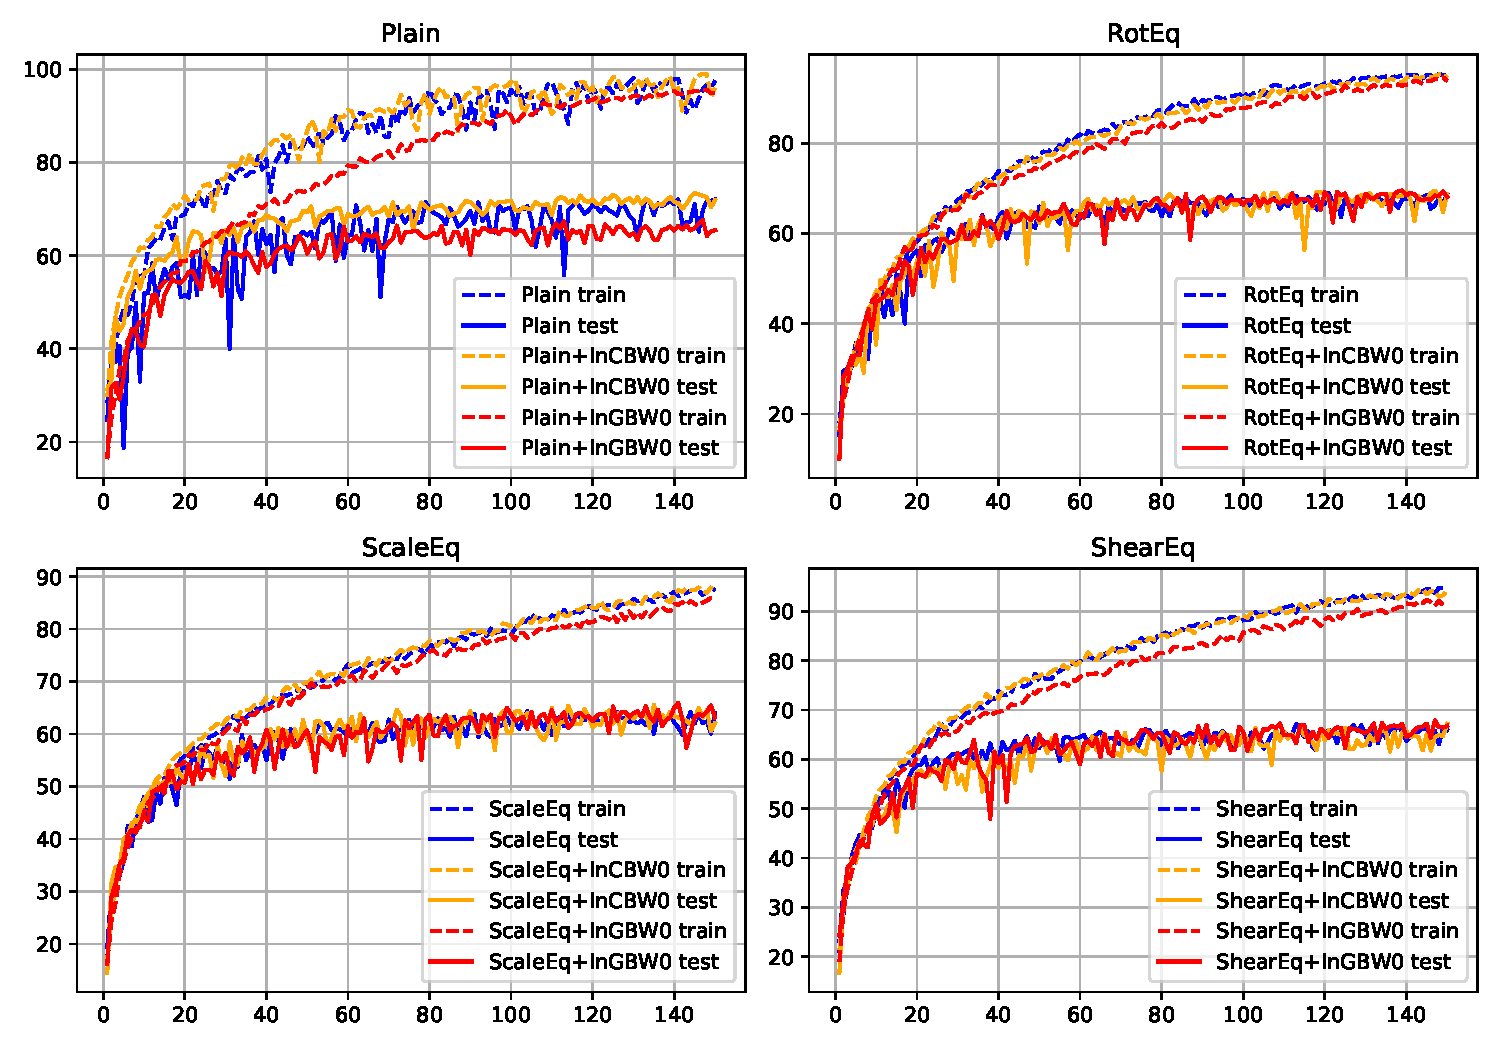
\includegraphics[width=0.85\textwidth]{plots/plot2/stl10}
        \caption{Comparison of classification accuracy of base models and their
            invariant versions on STL10 dataset.}
        \label{fig:plot2stl10}
    \end{figure}
    \begin{figure}[h!]
        \centering
        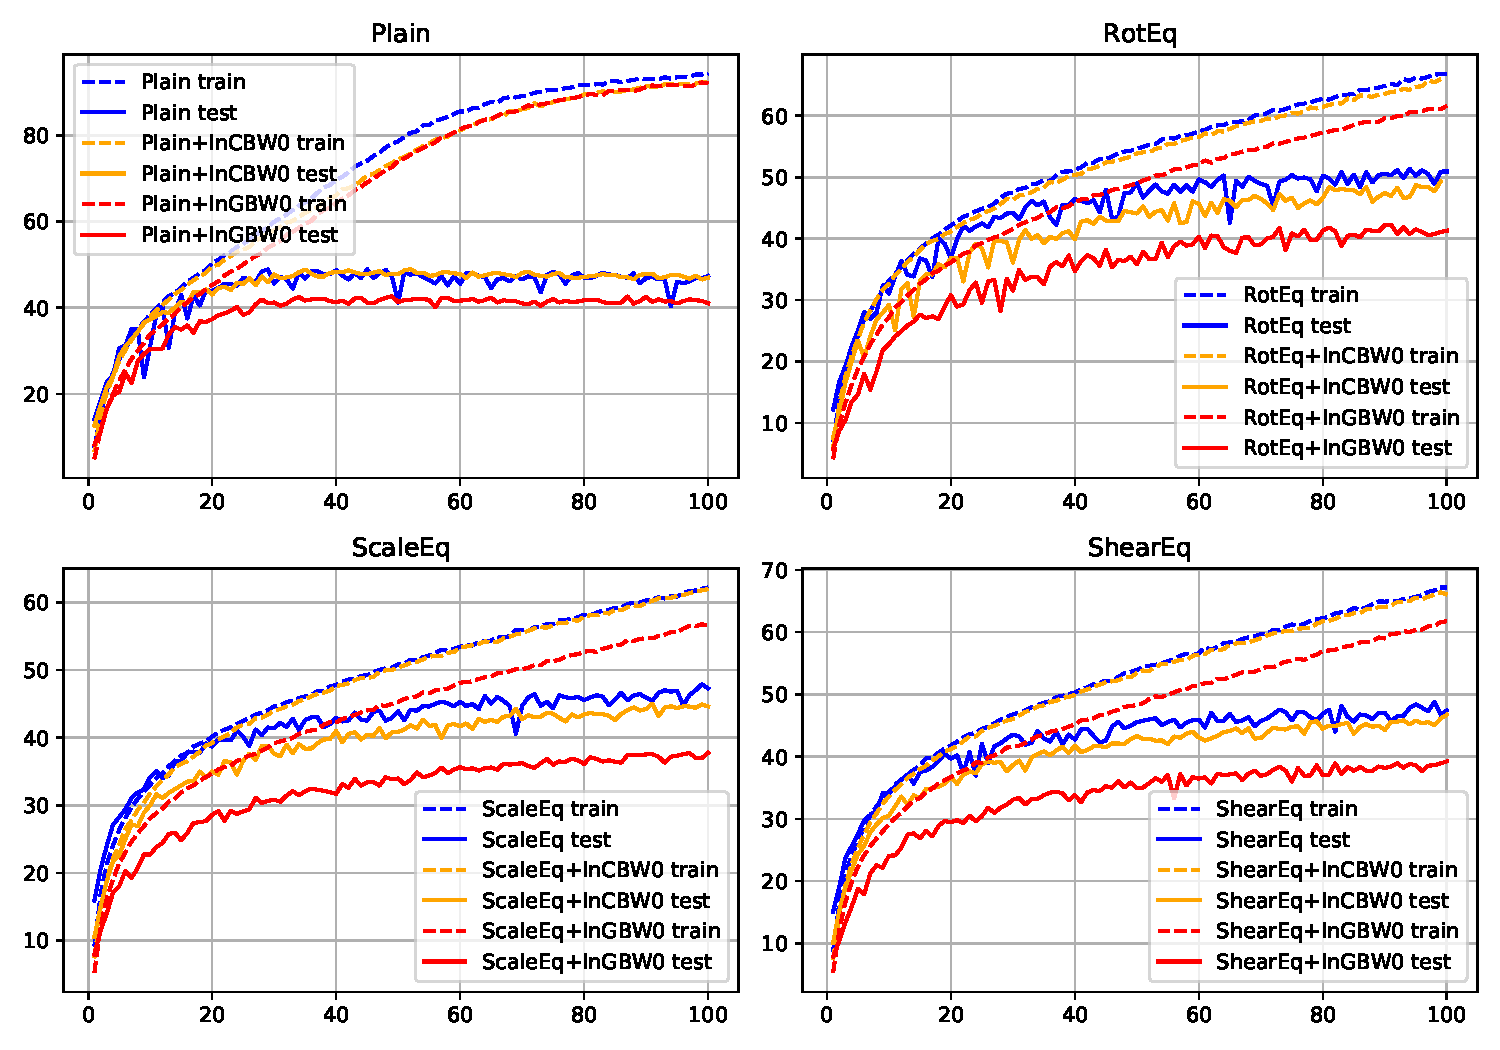
\includegraphics[width=0.85\textwidth]{plots/plot2/cifar100}
        \caption{Comparison of classification accuracy of base models and their
            invariant versions on CIFAR100 dataset.}
        \label{fig:plot2cifar100}
    \end{figure}
    \begin{figure}[h!]
        \centering
        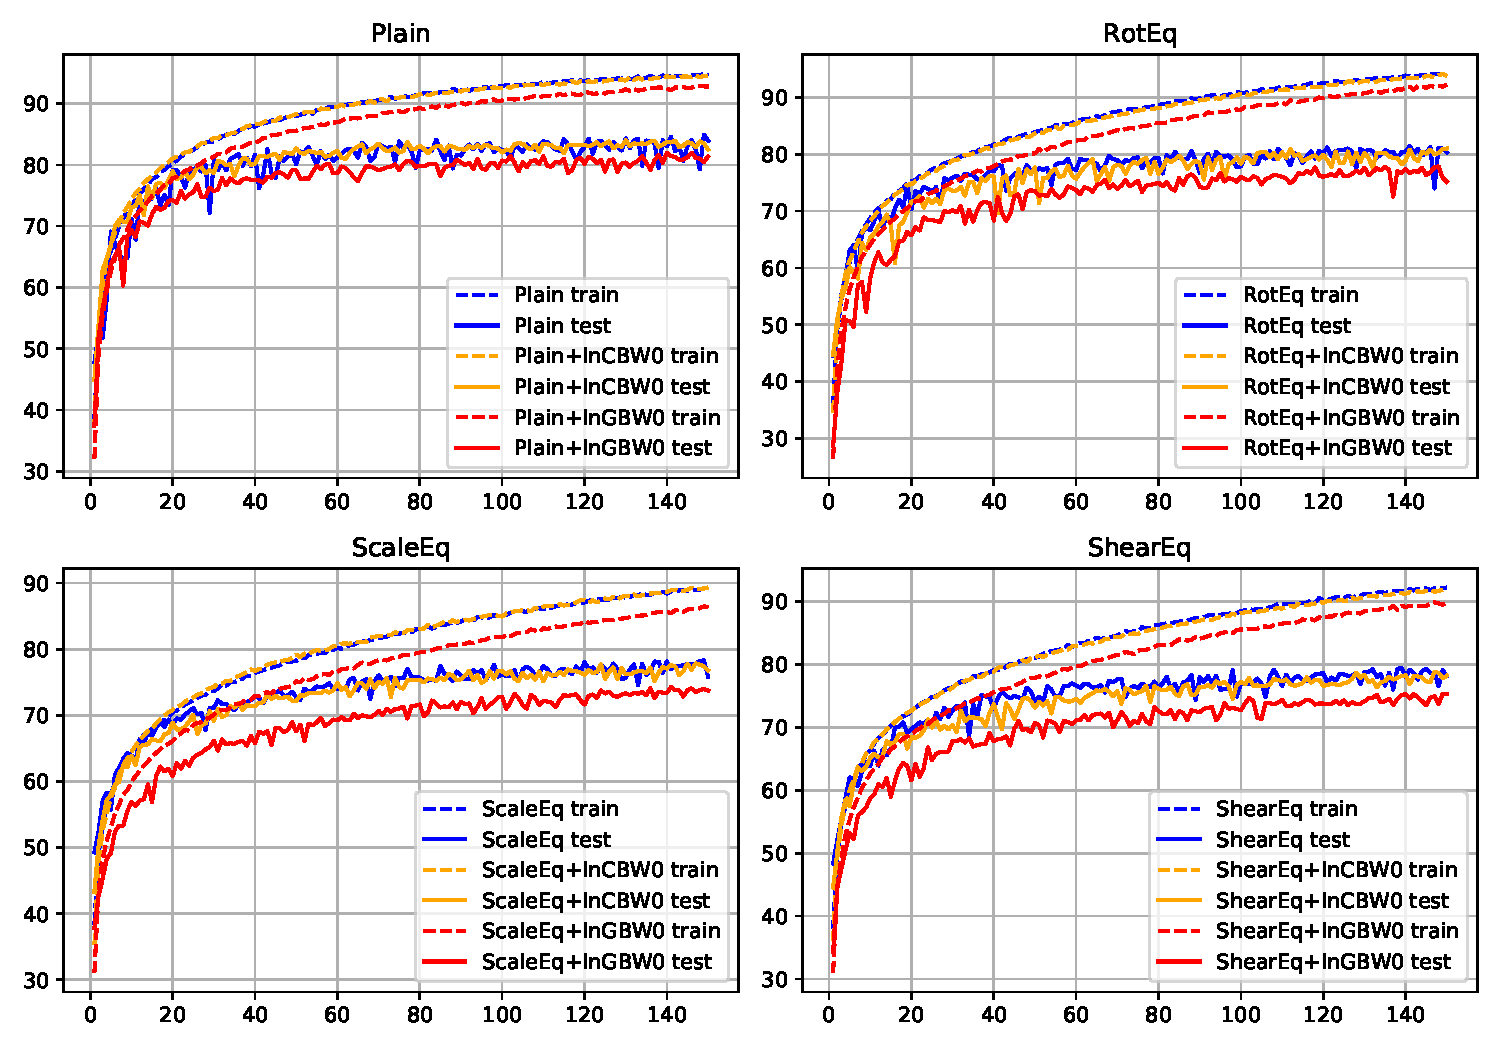
\includegraphics[width=0.85\textwidth]{plots/plot2/cifar10}
        \caption{Comparison of classification accuracy of base models and their
            invariant versions on CIFAR10 dataset.}
        \label{fig:plot2cifar10}
    \end{figure}




    %%%%%%%% brightnessEq, inb1, inb3, inb5 %%%%%%
    \subsubsection*{Comparison of brightness invariant models}
    Differences between architectures invariant and
    equivariant to changes in brightness are shown in figure \ref{fig:plot3}.
    To be precise BrightnessEq isn't
    exactly equivariant -- it's last fully-connected layer isn't equivariant due
    to bias vector. In classification problem however, what's important
    is that significant portion of the network exhibits equivariant behaviour.
    By that logic though model InB5 should also probably called equivariant as
    it's first $4$ residual bottlenecks are equivariant. All in all boundary
    between invariance and equivariance in NN literature is fluid and one should
    always pay attention what is meant by these terms. This particular is best
    interpreted as asking whether depth at which network becomes invariant plays
    any role. The answer to this question seems to be yes, but only if the task
    is sufficiently hard.

    Starting with the easiest CIFAR10 dataset we see test accuracy of all models
    differs only slightly, though it's worth noting that InB1 is ahead of others
    for most of the training time. Training curves on the other hand reveal
    significant difference of training speed of InB1 and BrightnessEq.

    In CIFAR100 experiments the differences are more pronounced. InB1 clearly
    dominates the rest, while InB5 and BrightnessEq are the lest accurate.
    It's test curve is becomes stable after $50$th epoch whereas InB5's doesn't.
    Training plots confirm as well that InB1 and InB3 are able to optimize the
    fastest.

    InB5 does relatively poorly also on STL10. Curiously, skipping BrightnessEq,
    it's the Plain model whose training curve is the most jarred

    Overall InB1 network seems to slightly outperform the default Plain+InCBW0
    model.
    The only difference between them is availability of the
    brightness information to the first two convolutional layers and
    intermediate ReLU activation. This might help InB1 to differentiate between
    classes if the interclass variation of brightness is significant. This
    turns out to be true
    for CIFAR100 but not really for CIFAR10 and STL10 (see figure
    \ref{fig:plot3brightness}), which could explain big differences in
    performance between individual networks on the first dataset.



    \begin{figure}[h!]
        \centering
        \includegraphics[width=\textwidth]{plots/plot3/plot}
        \caption{Comparison of classification accuracy of
        brightness equivariant and invariant models.}
        \label{fig:plot3}
    \end{figure}

    \begin{figure}[h!]
        \centering
        \begin{subfigure}{0.7\textwidth}
            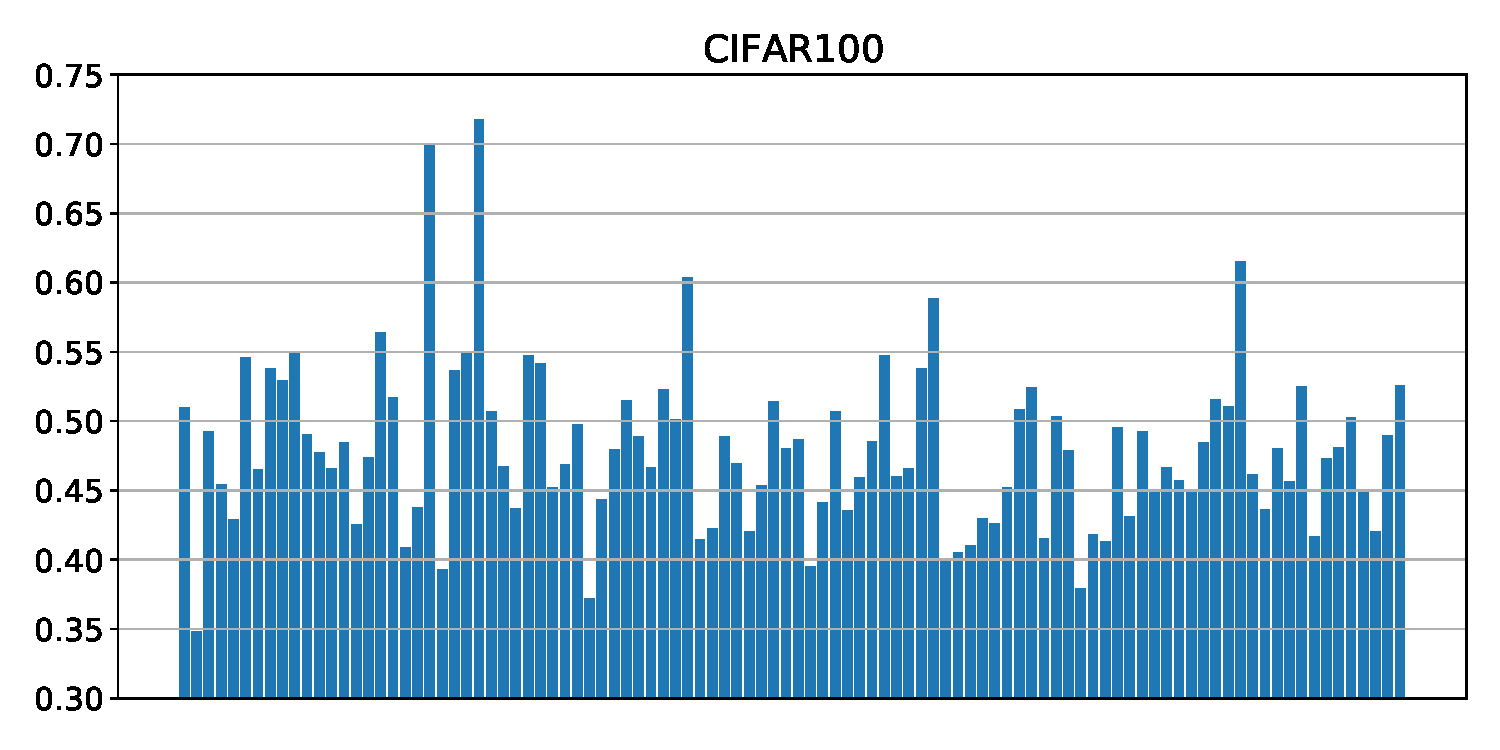
\includegraphics[width=\linewidth]{plots/plot3/cifar100_br}
        \end{subfigure}
        \begin{subfigure}{0.45\textwidth}
            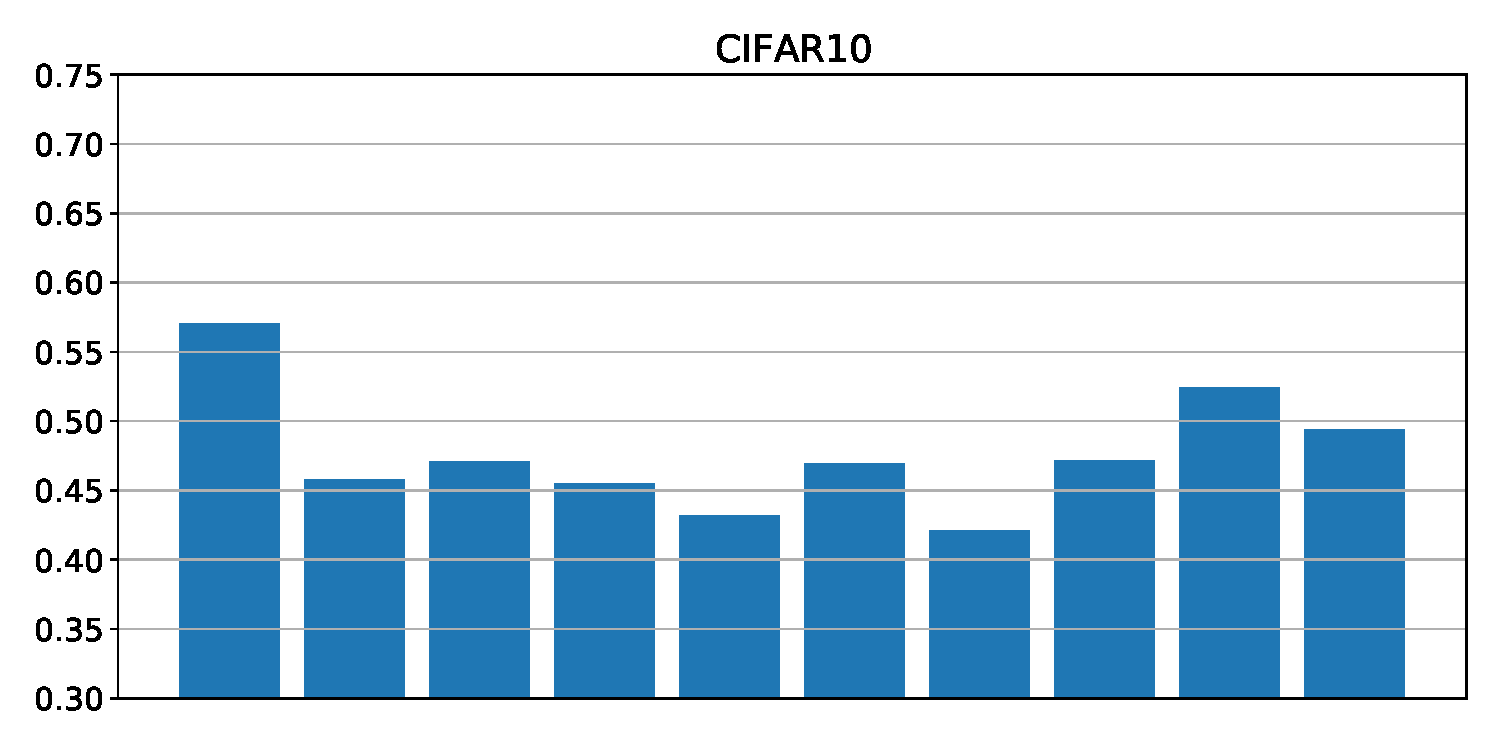
\includegraphics[width=\linewidth]{plots/plot3/cifar10_br}
        \end{subfigure}
        \begin{subfigure}{0.45\textwidth}
            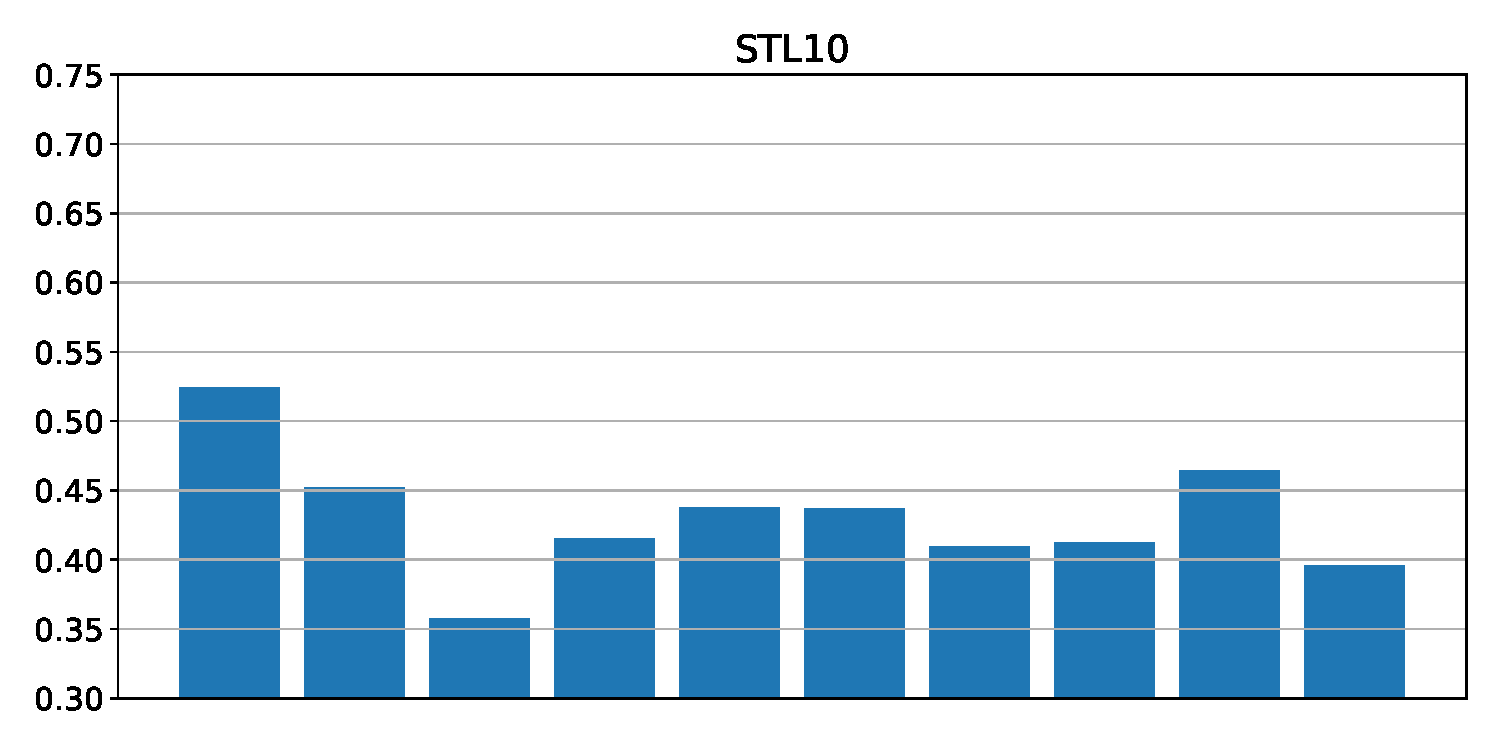
\includegraphics[width=\linewidth]{plots/plot3/stl10_br}
        \end{subfigure}
        \caption{Mean brightness of every class in CIFAR100, CIFAR10 and STL10
            datasets as measured on test parts.}
        \label{fig:plot3brightness}
    \end{figure}

    %%%%%%%%% top 5 best %%%%%%%%%%%%%%%%%%%%%%%%%%
    \clearpage
    \subsubsection*{Comparison of top networks}
    \begin{figure}[h!]
        \centering
        \includegraphics[width=\textwidth]{plots/plot5/plot}
        \caption{Comparison of classification accuracy of
            5 best models for each dataset.
            Models were ranked according to maximum test set accuracy during
            training.}
        \label{fig:plot5}
    \end{figure}

    %%%%% jitter vs non-jitter %%%%%%%%%%
    \clearpage
    \subsubsection*{Effectiveness of data augmentation}
        \begin{table}
        \centering
        \begin{tabular}{|c|c|c|}
         \hline
         Model name & No augmentation & Augmentation \\
         \hline
            Plain & {84.9} & {84.5} \\
            Plain+InCBW0 & {84.0} & {84.9} \\
            Plain+InGBW0 & {82.0} & {82.1} \\
            RotEq & {81.5} & {81.3} \\
            RotEq+InCBW0 & {81.0} & {80.9} \\
            RotEq+InGBW0 & {77.9} & {79.5} \\
            ScaleEq & {78.3} & {77.9} \\
            ScaleEq+InCBW0 & {77.8} & {78.5} \\
            ScaleEq+InGBW0 & {74.3} & {74.9} \\
            SchearEq & {79.4} & {78.9} \\
            SchearEq+InCBW0 & {78.8} & {79.3} \\
            SchearEq+InGBW0 & {75.3} & {77.0} \\
            GammaEq & {76.7} & {76.4} \\
            BrightnessEq & {83.3} & {82.9} \\
            InB1 & {84.5} & {84.5} \\
            InB2 & {84.0} & {83.1} \\
            InB3 & {84.2} & {83.9} \\
         \hline
        \end{tabular}
        \caption{Comparison of classification accuracy on CIFAR10 with an without
            data augmentation.}
        \label{tab:jitter_table}
        \end{table}

    %%%%% generalizations %%%%%%%%%%%%%%%
    \clearpage
    \subsubsection*{Generalizations}
    Matrices in figures \ref{fig:plot4brightness}, \ref{fig:plot4contrast},
    \ref{fig:plot4gamma} and \ref{fig:plot4color} illustrate robustness of trained
    models to brightness, contrast, gamma and color balance transformations
    respectively. Specifically the test part of dataset is first passed through
    a transform, the network then classifies transformed images and accuracy of
    prediction is measured. Matrices contain accuracies expressed in percentages.

    In \ref{fig:plot4gamma} and \ref{fig:plot4color} images are converted
    precisely according to $\mathcal{G}$ (equation \ref{eq:gamma})
    and $\mathcal{W}$ (equation \ref{eq:color}) operators. $\mathcal{C}$
    (eq \ref{eq:contrast})
    and $\mathcal{B}$ (eq \ref{eq:bright}) symmetries are in turn additionally
    clipped to $[0;1]$ range so that their results are still viewable images.
    There's a lot of data to analyze, but conclusions mostly carry over between
    datasets.

    Starting with base Plain model we observe radical changes in brightness
    are heavily detrimental to networks' performance, wherein darkening image
    is more impactful. This might be consequence of clipping -- lowering
    brightness causes mean value of input to decrease linearly, while increasing
    causes sublinear growth. The same phenomenon occurs in case of contrast and
    color balance changes. The network is on the other hand far more resistant
    \begin{figure}[h!]
    \begin{adjustwidth}{-11em}{-11em}
        \centering
        \begin{subfigure}{0.6\textwidth}
            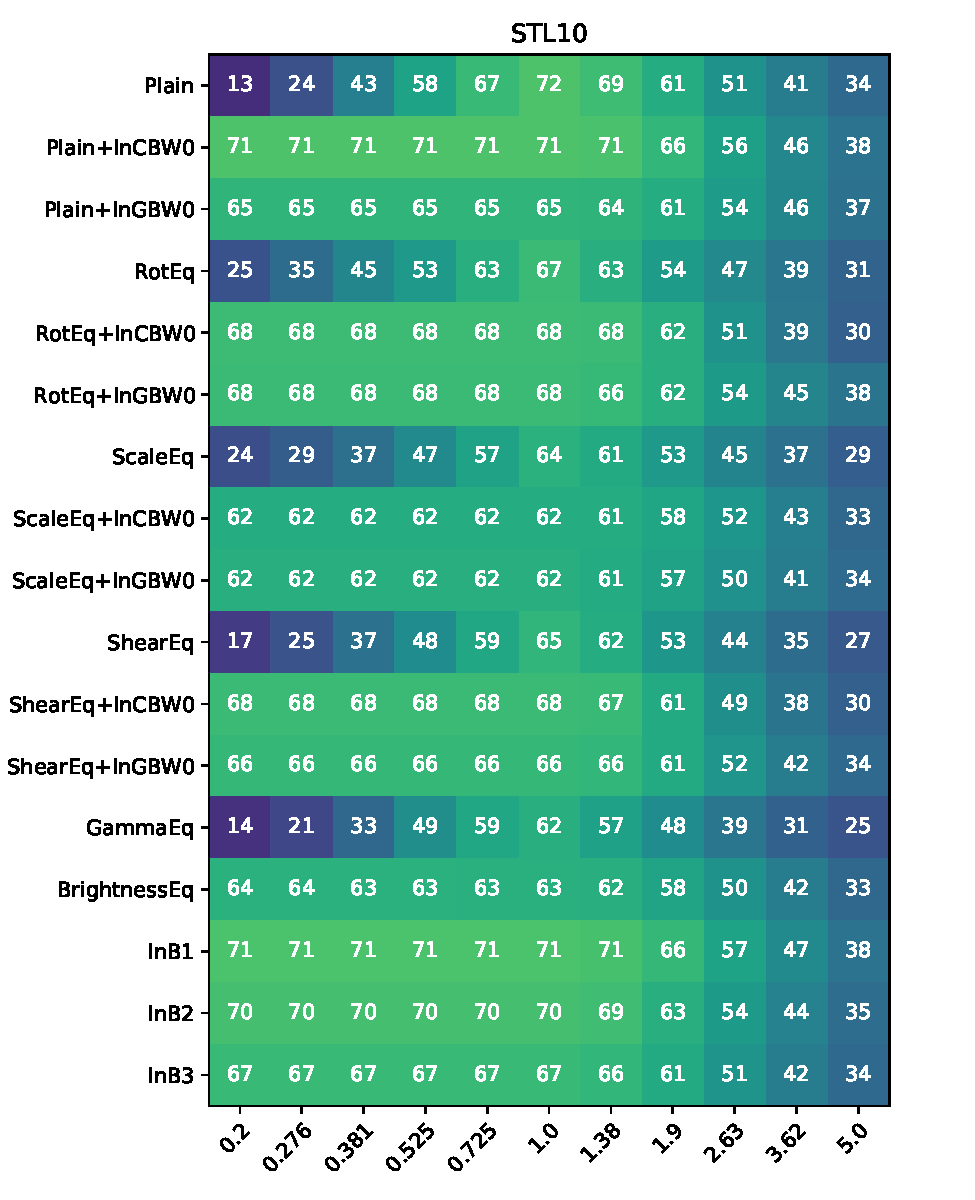
\includegraphics[width=\linewidth]{plots/plot4/brightness_stl10}
        \end{subfigure}
        \begin{subfigure}{0.6\textwidth}
            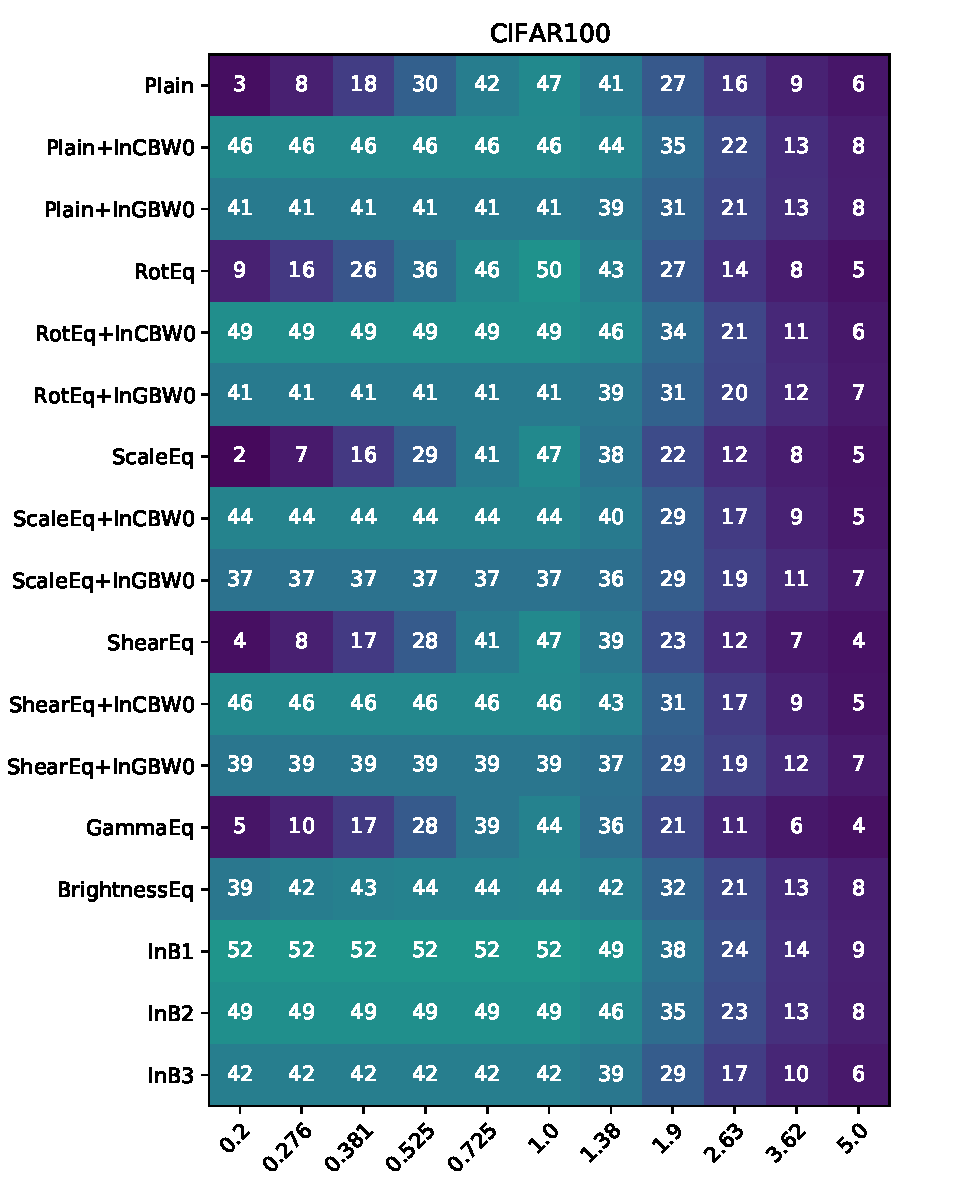
\includegraphics[width=\linewidth]{plots/plot4/brightness_cifar100}
        \end{subfigure}
        \begin{subfigure}{0.6\textwidth}
            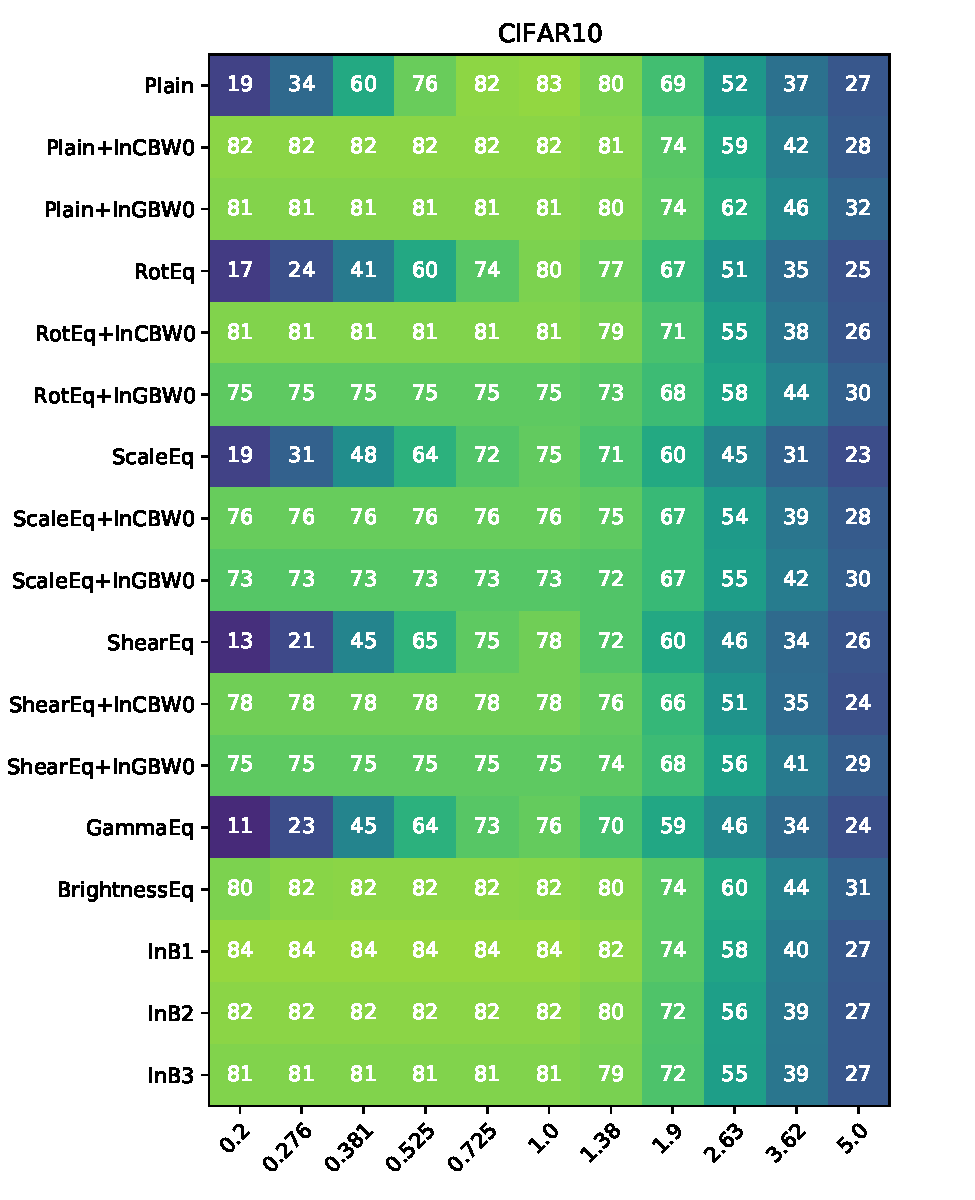
\includegraphics[width=\linewidth]{plots/plot4/brightness_cifar10}
        \end{subfigure}
        \begin{subfigure}{0.6\textwidth}
            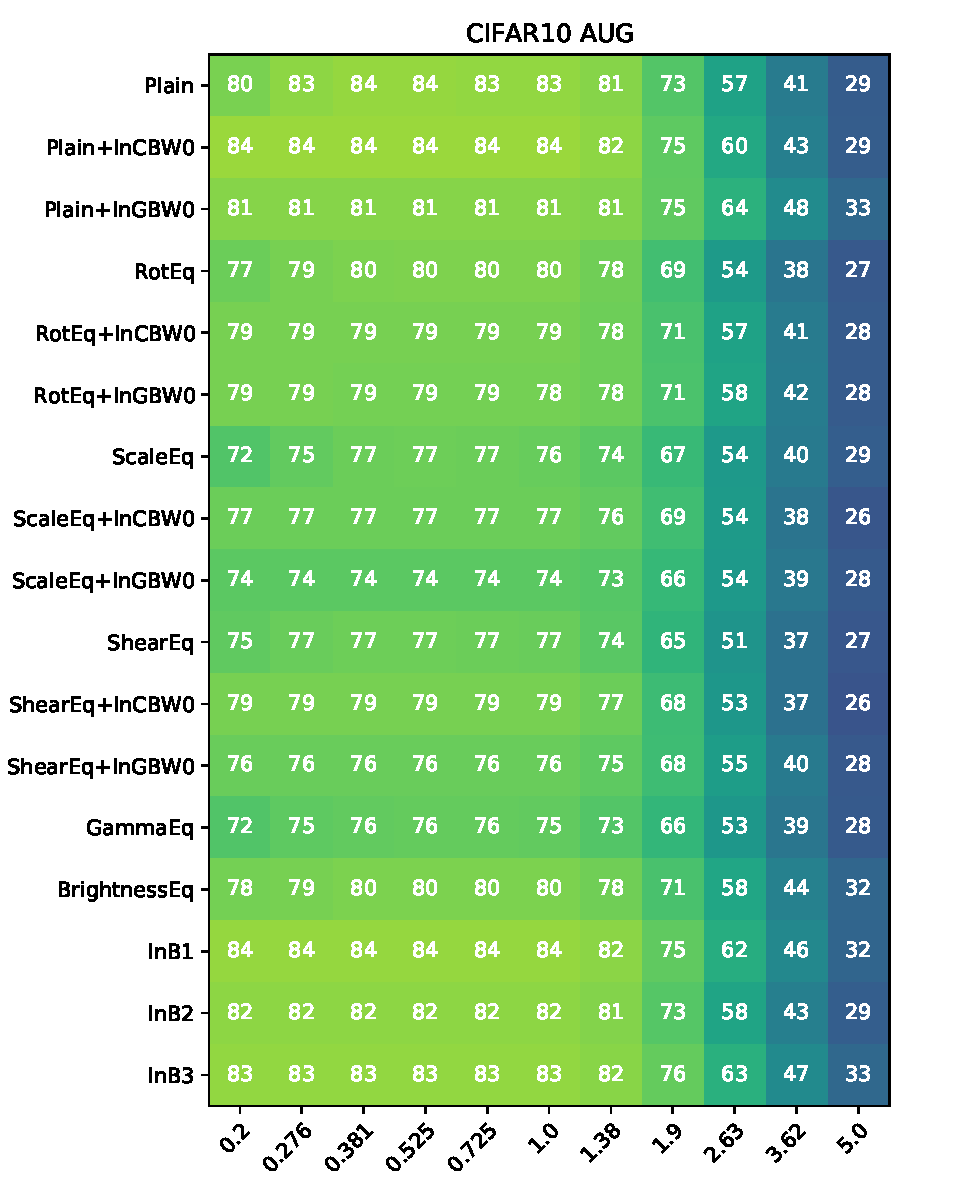
\includegraphics[width=\linewidth]{plots/plot4/brightness_cifar10_jitter}
        \end{subfigure}
    \end{adjustwidth}
        \caption{Classification accuracy of each model depending on the change
        of brightness $\mathcal{B}_a$ in input. X axis indicates value of
        parameter $a$.}
        \label{fig:plot4brightness}
    \end{figure}


    \begin{figure}[h!]
    \begin{adjustwidth}{-11em}{-11em}
        \centering
        \begin{subfigure}{0.6\textwidth}
            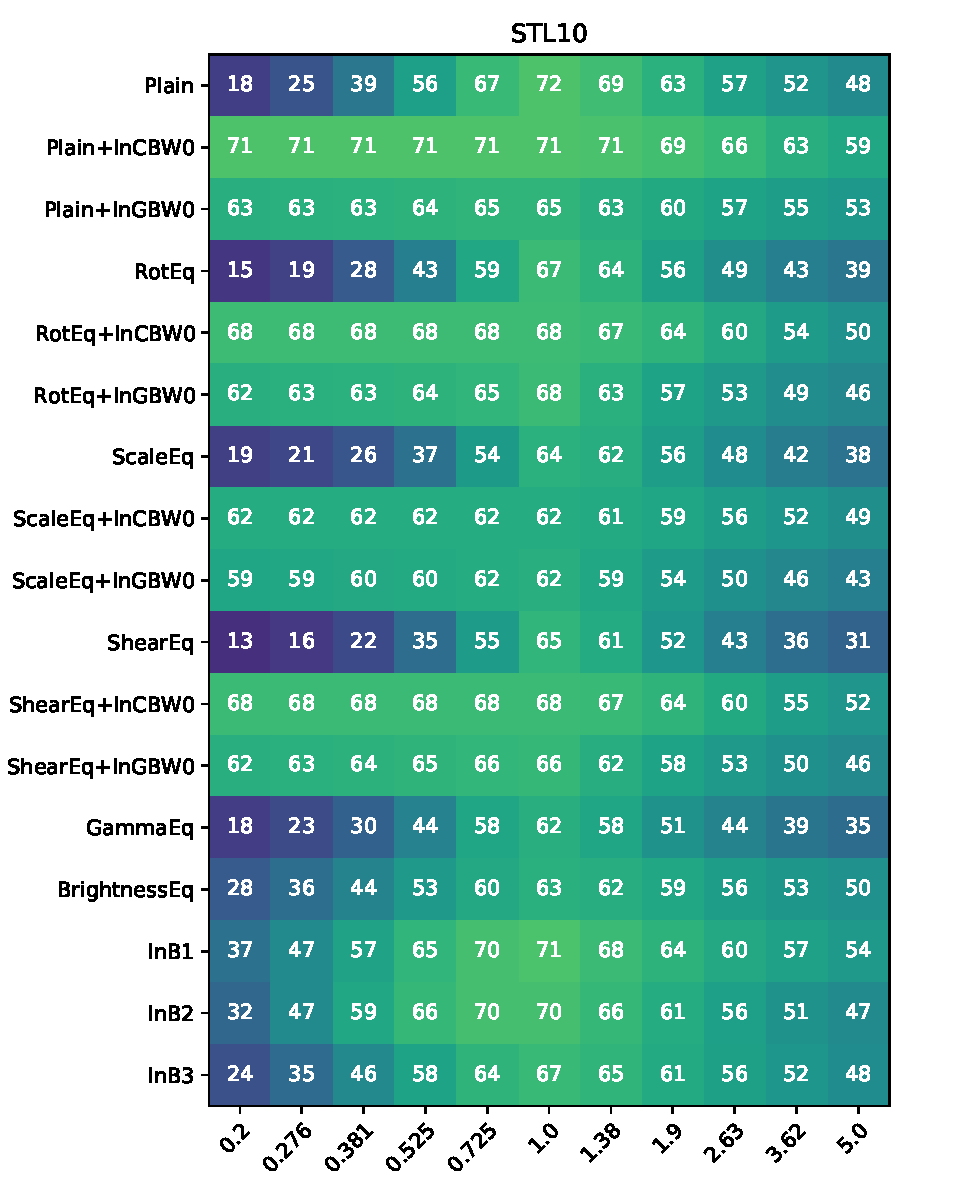
\includegraphics[width=\linewidth]{plots/plot4/contrast_stl10}
        \end{subfigure}
        \begin{subfigure}{0.6\textwidth}
            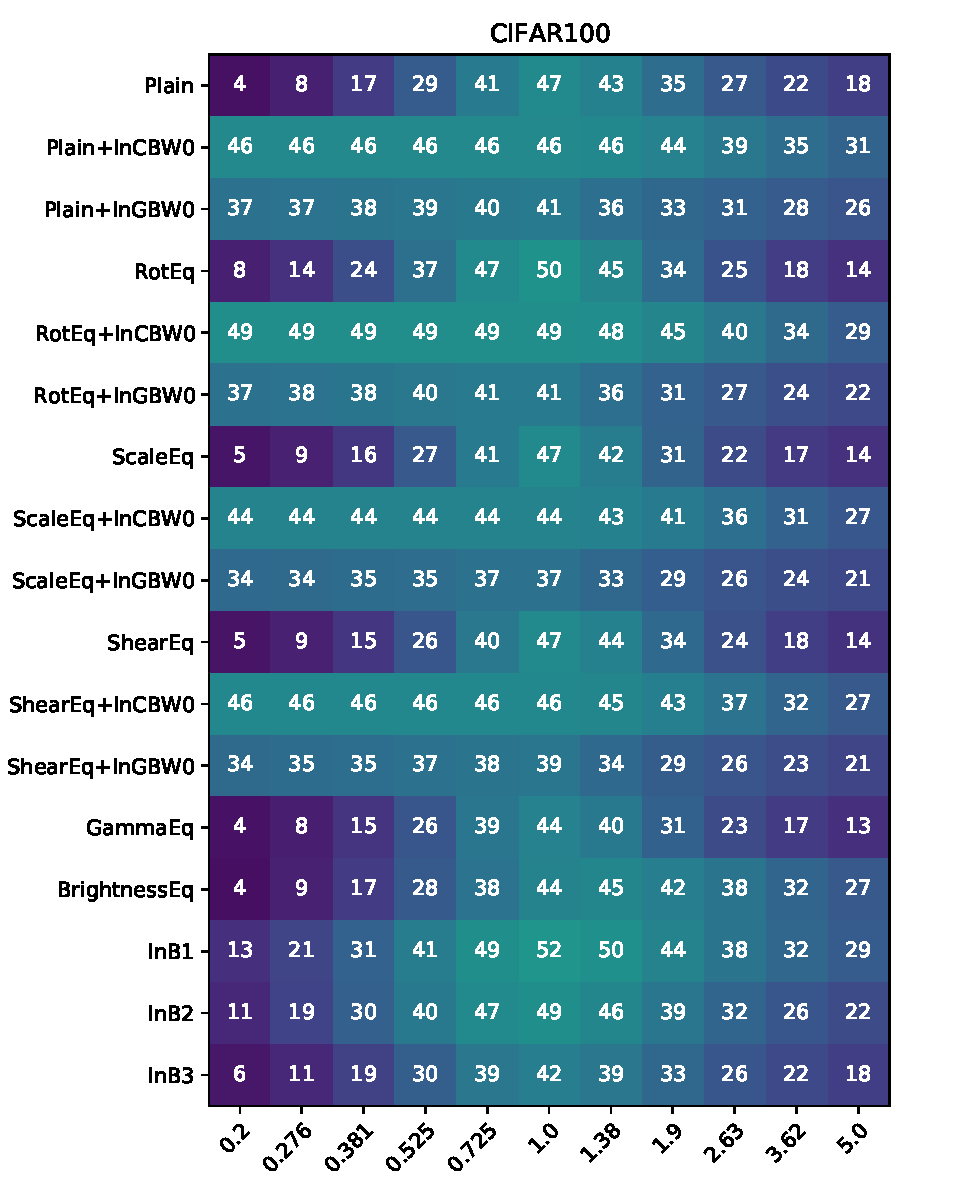
\includegraphics[width=\linewidth]{plots/plot4/contrast_cifar100}
        \end{subfigure}
        \begin{subfigure}{0.6\textwidth}
            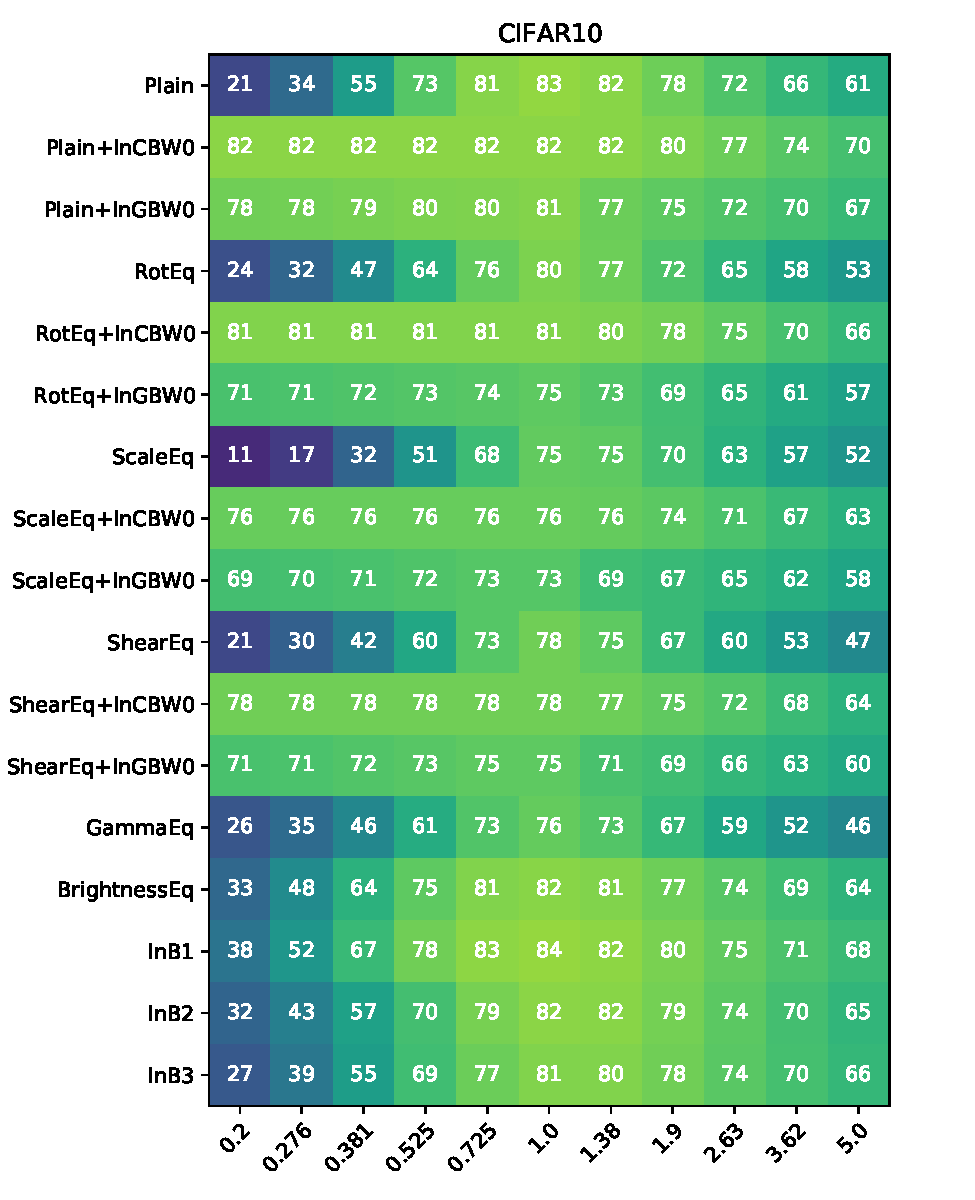
\includegraphics[width=\linewidth]{plots/plot4/contrast_cifar10}
        \end{subfigure}
        \begin{subfigure}{0.6\textwidth}
            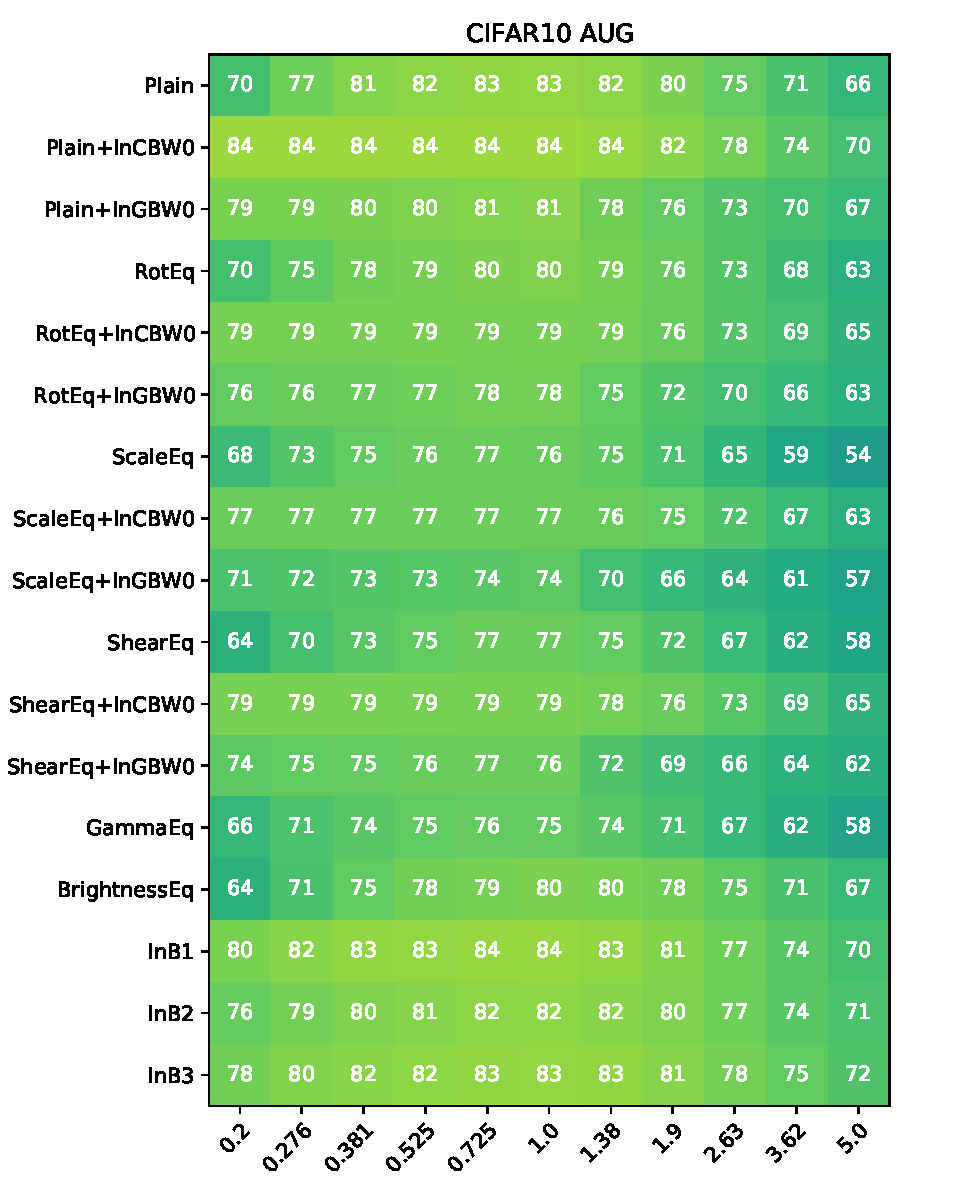
\includegraphics[width=\linewidth]{plots/plot4/contrast_cifar10_jitter}
        \end{subfigure}
    \end{adjustwidth}
        \caption{Classification accuracy of each model depending on the change
        of contrast $\mathcal{C}_c$ in input.}
        \label{fig:plot4contrast}
    \end{figure}


    \begin{figure}[h!]
    \begin{adjustwidth}{-11em}{-11em}
        \centering
        \begin{subfigure}{0.6\textwidth}
            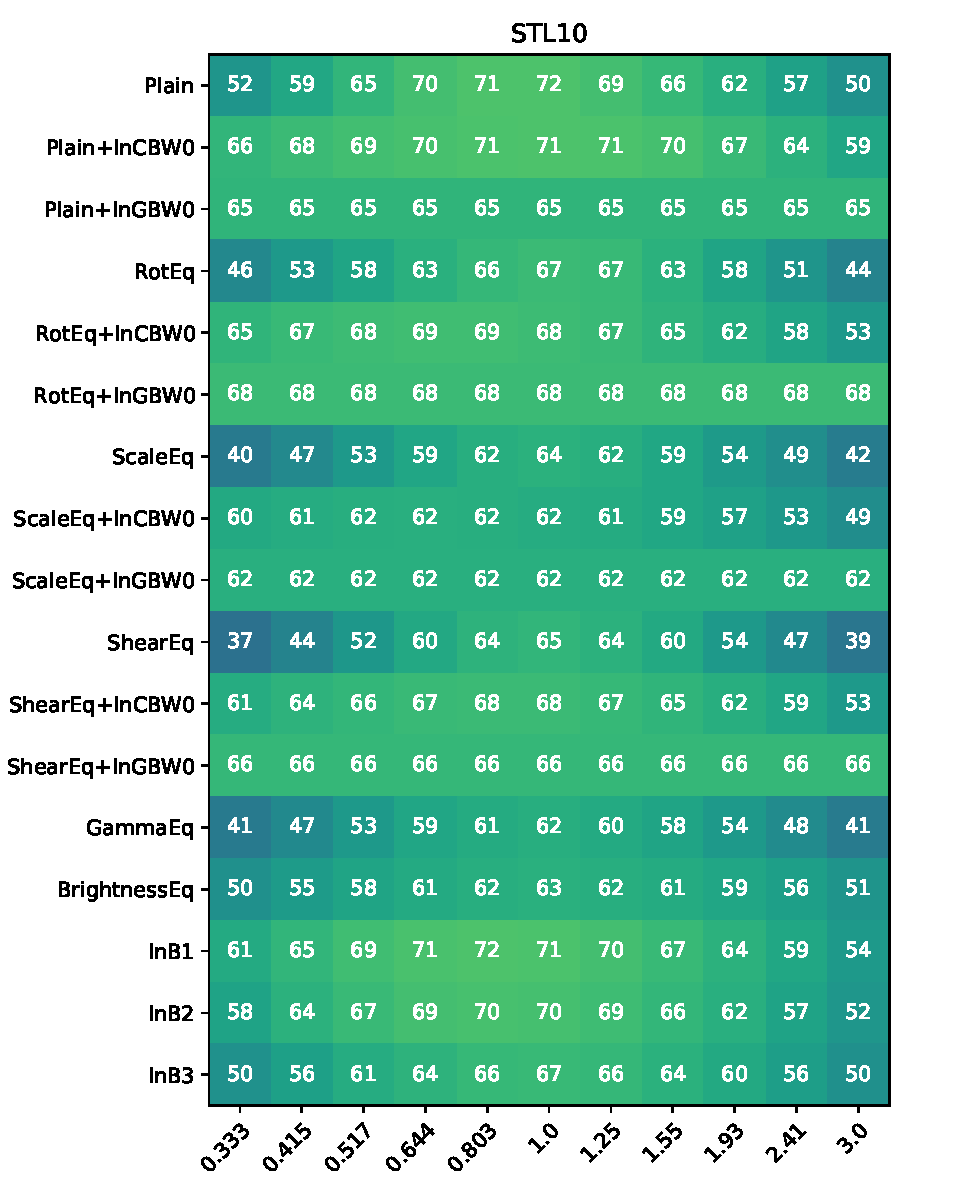
\includegraphics[width=\linewidth]{plots/plot4/gamma_stl10}
        \end{subfigure}
        \begin{subfigure}{0.6\textwidth}
            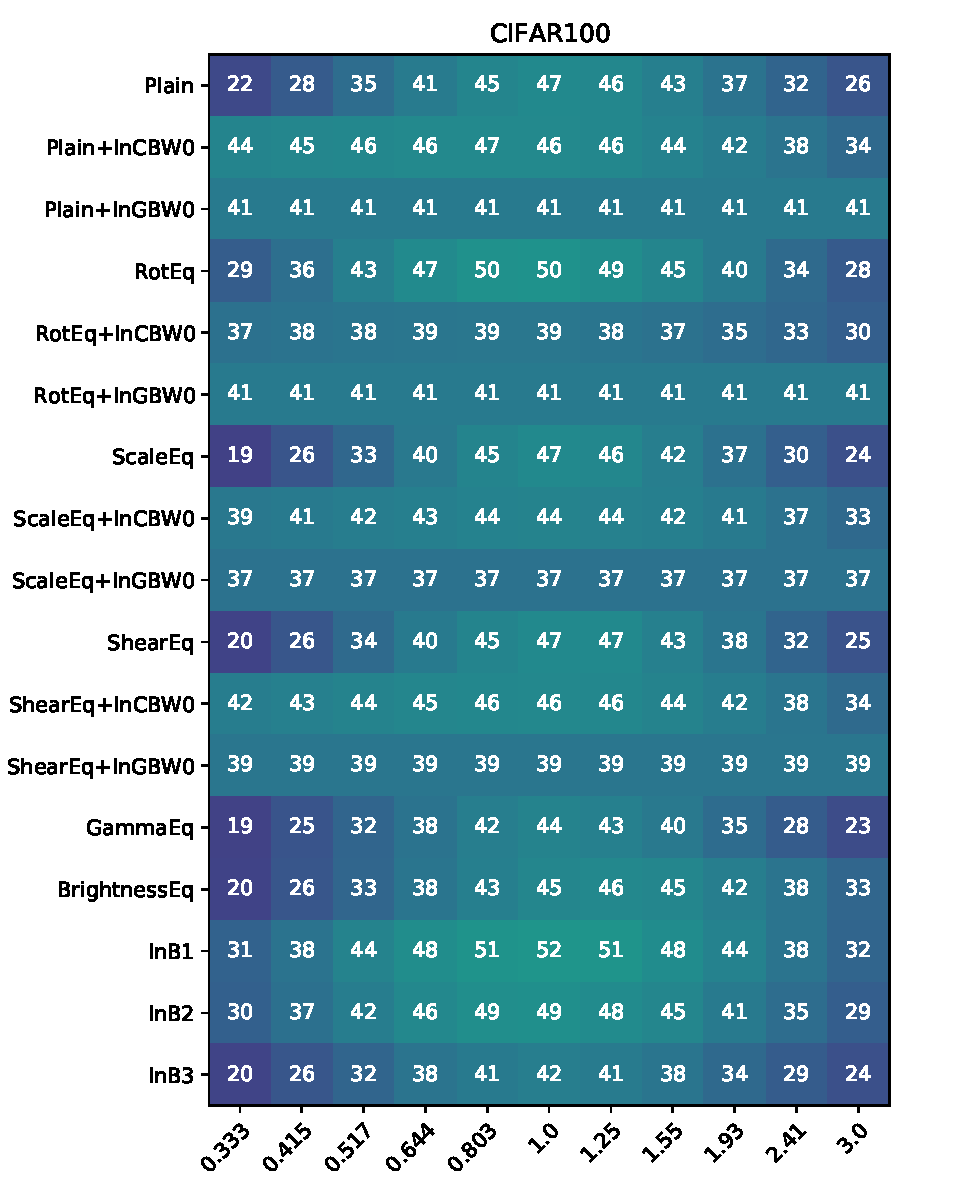
\includegraphics[width=\linewidth]{plots/plot4/gamma_cifar100}
        \end{subfigure}
        \begin{subfigure}{0.6\textwidth}
            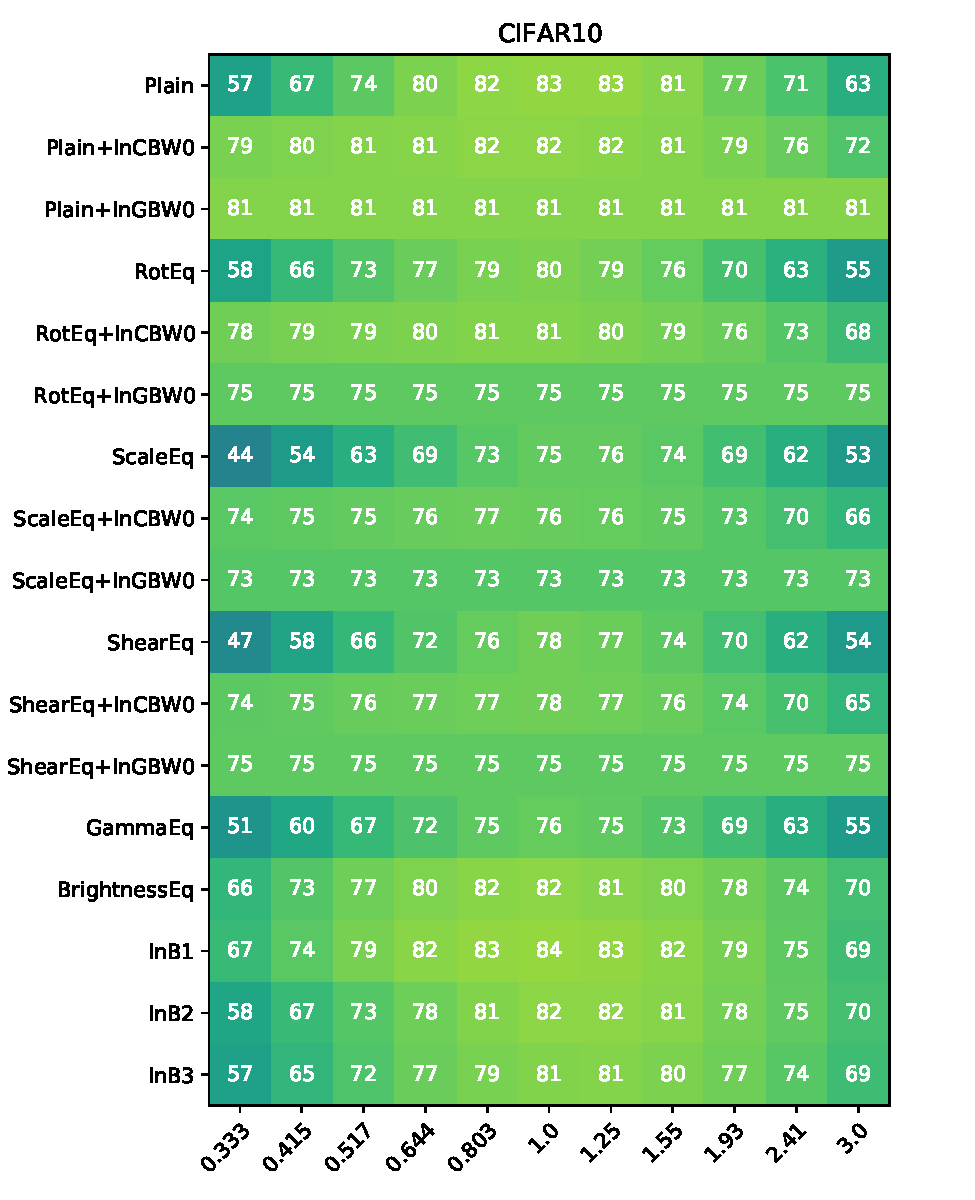
\includegraphics[width=\linewidth]{plots/plot4/gamma_cifar10}
        \end{subfigure}
        \begin{subfigure}{0.6\textwidth}
            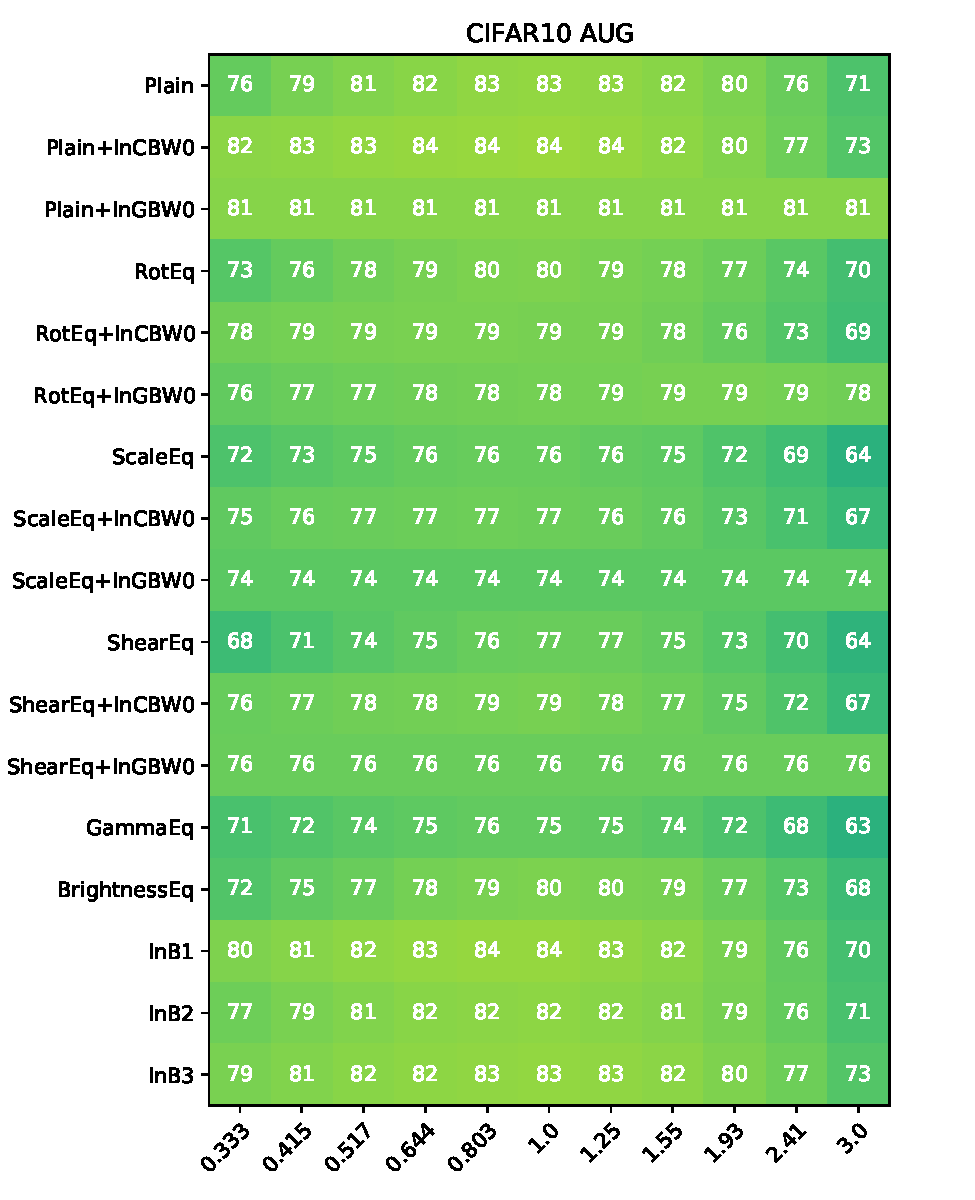
\includegraphics[width=\linewidth]{plots/plot4/gamma_cifar10_jitter}
        \end{subfigure}
    \end{adjustwidth}
        \caption{Classification accuracy of each model depending on the change
        of gamma $\mathcal{G}_c$ in input.}
        \label{fig:plot4gamma}
    \end{figure}


    \begin{figure}[h!]
    \begin{adjustwidth}{-11em}{-11em}
        \centering
        \begin{subfigure}{0.6\textwidth}
            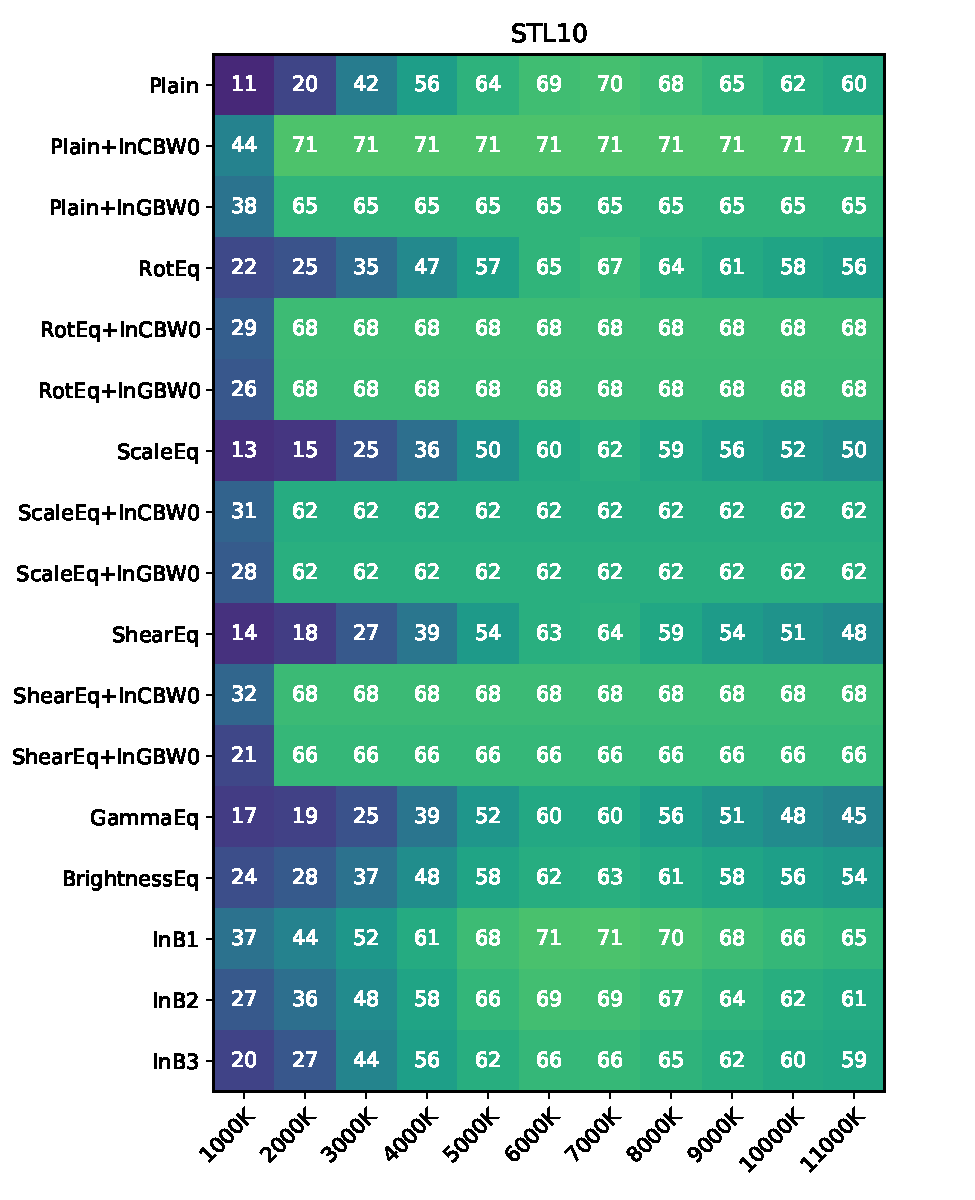
\includegraphics[width=\linewidth]{plots/plot4/color_stl10}
        \end{subfigure}
        \begin{subfigure}{0.6\textwidth}
            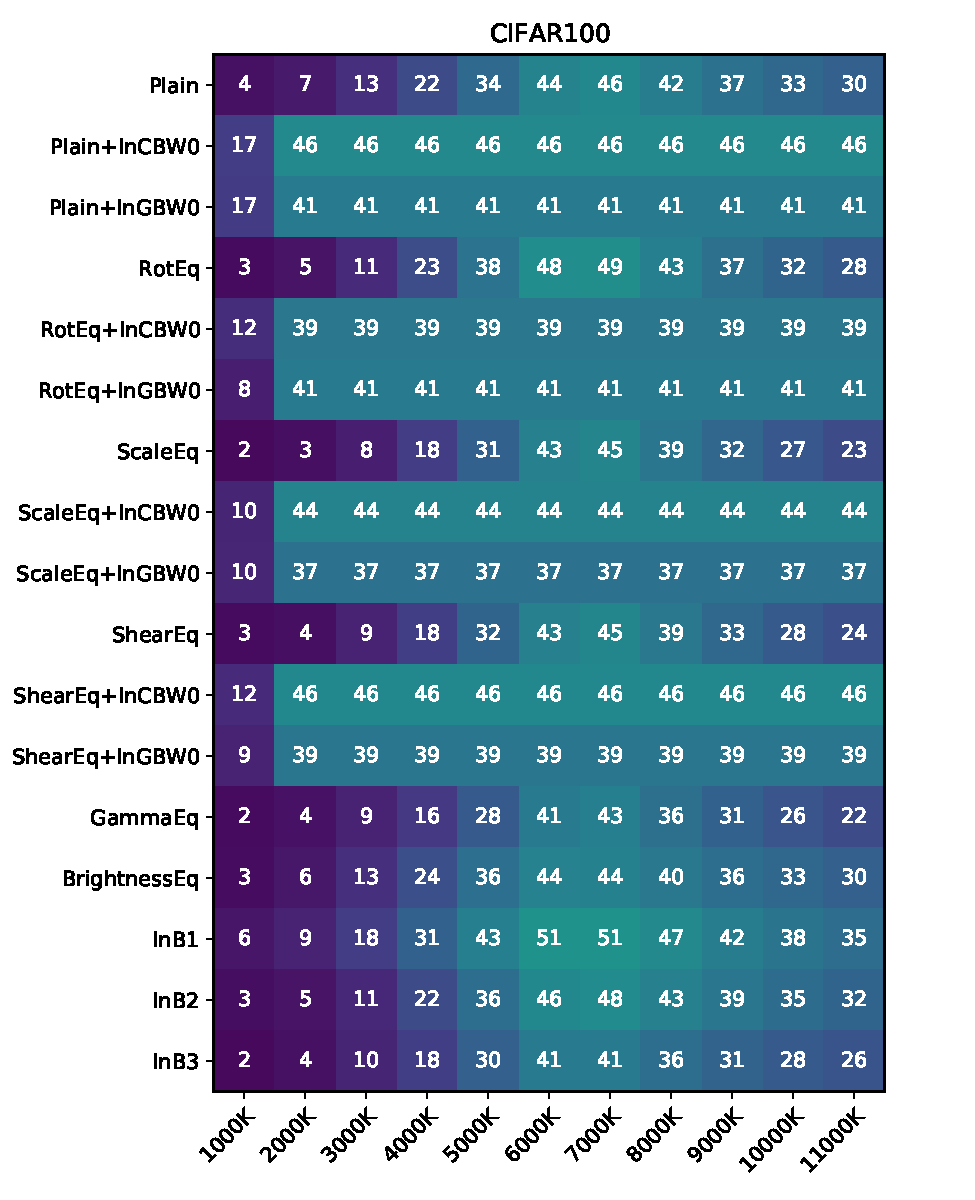
\includegraphics[width=\linewidth]{plots/plot4/color_cifar100}
        \end{subfigure}
        \begin{subfigure}{0.6\textwidth}
            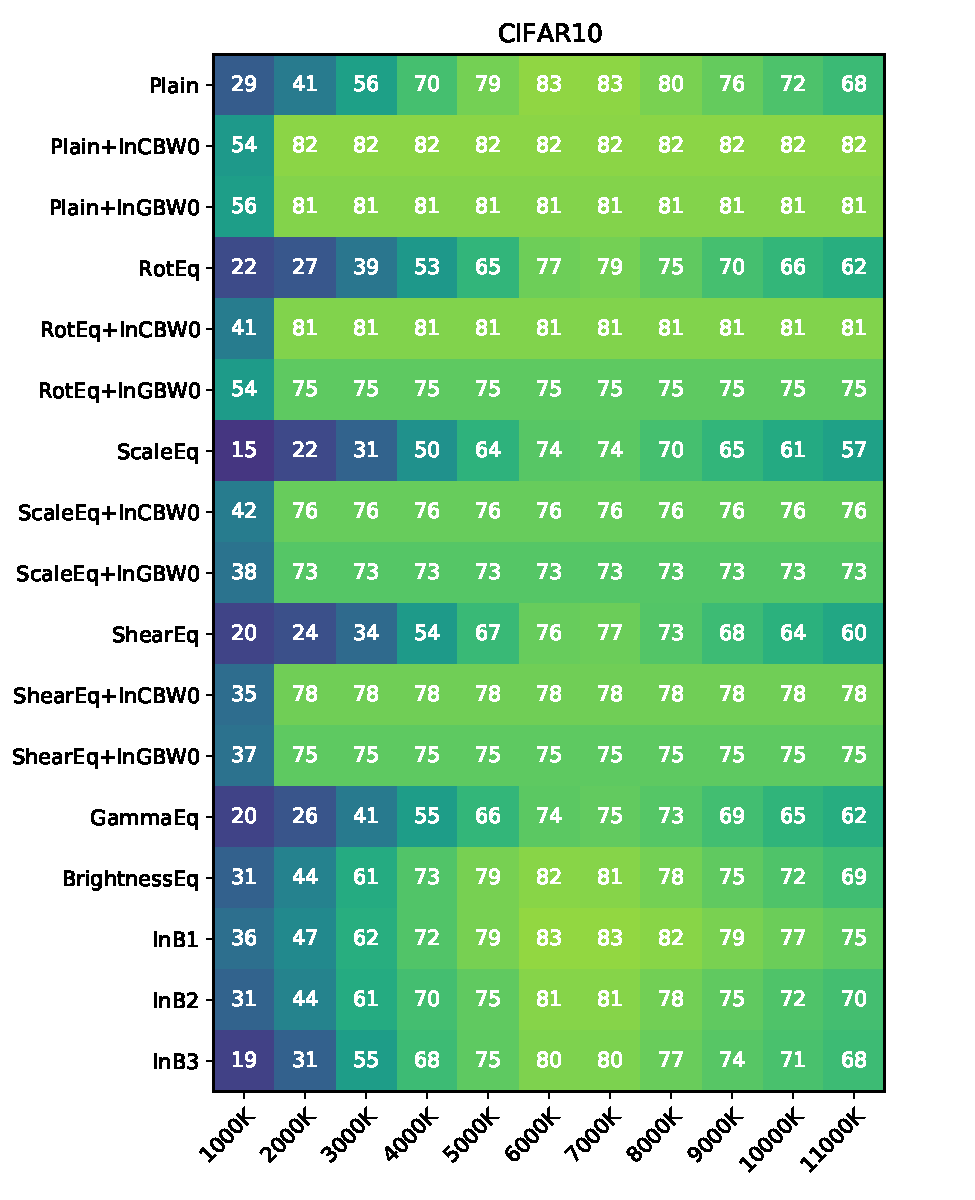
\includegraphics[width=\linewidth]{plots/plot4/color_cifar10}
        \end{subfigure}
        \begin{subfigure}{0.6\textwidth}
            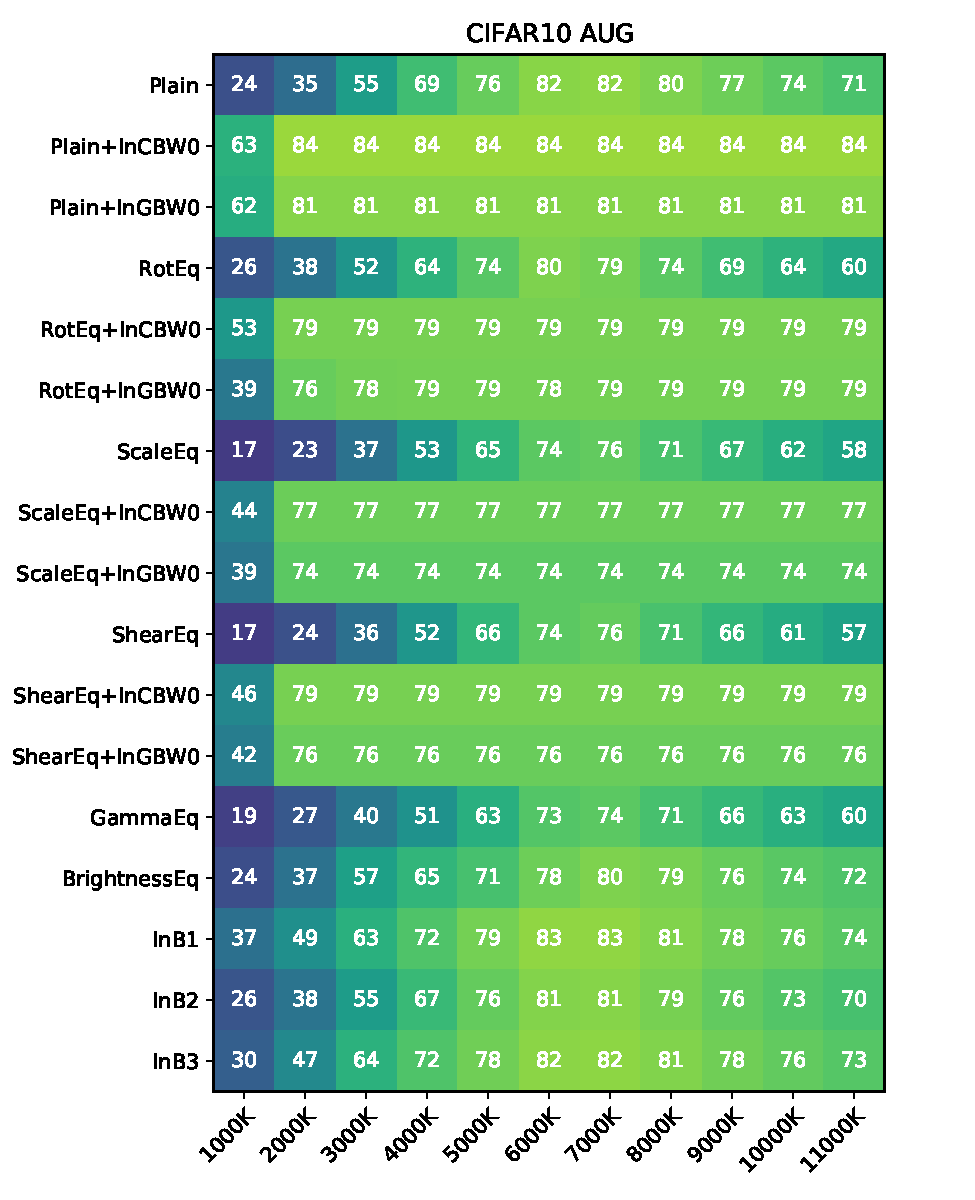
\includegraphics[width=\linewidth]{plots/plot4/color_cifar10_jitter}
        \end{subfigure}
    \end{adjustwidth}
        \caption{Classification accuracy of each model depending on the change
        of color balance $\mathcal{W}_T$ in input.}
        \label{fig:plot4color}
    \end{figure}

    %%%%%% equivariance %%%%%%%%%%%%%
\clearpage
\subsection{Degree of equivariance and invariance}
    \newcommand{\mcn}{\mathcal{N}}
    \newcommand{\mct}{\mathcal{T}}
    Now we investigate degree of equivariance present at
    various depths of networks. While modern literature of GCNNs builds on
    thorough theoretical framework, claims of theoretical properties are hardly
    ever checked directly. \cite{attentive_gcnn} compares attention fields
    produced by equivariant attention mechanism visually.
    Of all papers cited in bibliography the only one containing numerical
    experiments is
    \cite{scale_steerable} where equivariance to scaling is measured.
    We reformulate slightly the definition of relative error used in
    \cite{scale_steerable} to make it symmetric.
    Let $\mcn_k$ be the $k$th layer of
    the network and $\mcn_{k:0} = \mcn_k \circ \dots \circ \mcn_0$. Then the
    equivariance error of network $\mcn$
    at depth $k$ with respect to transformation $\mathcal{T}$
    and input $x$ equals
    $$ E_{\mcn_k,\mct}(x) = 2\frac{\left|\mcn_{k:0}\left(\mct(x)\right) -
    \mct(\mcn_{k:0}(x))\right|}
    {\left|\mcn_{k:0}(\mct(x))\right| + \left|\mct(\mcn_{k:0}(x))\right|} $$
    The total error is average across all images in dataset $X$:
    $$ E_{\mcn_k,\mct} = \frac{1}{|X|}\sum_{x \in X }E_{\mcn_k,\mct}(x) $$
    Matrices in figures
    \ref{fig:plot7brightness},
    \ref{fig:plot7gamma},
    \ref{fig:plot7rot},
    \ref{fig:plot7scale},
    \ref{fig:plot7shear},
    show errors measured for networks trained on CIFAR10 dataset.
    In each pair the left matrix shows error of base Plain model and the right one
    error of supposedly equivariant network.



    \begin{figure}[h!]
    \begin{adjustwidth}{-11em}{-11em}
        \centering
        \begin{subfigure}{0.4\textwidth}
            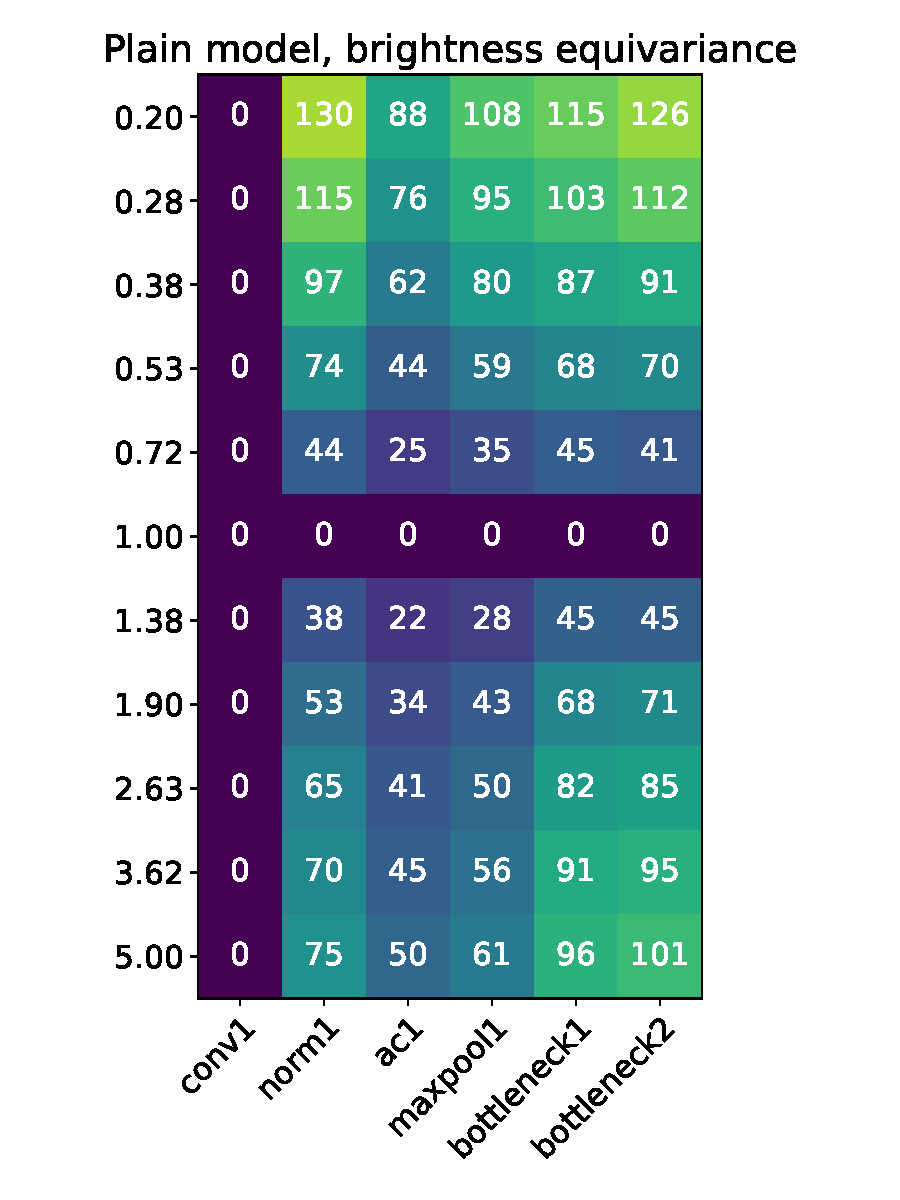
\includegraphics[width=\linewidth]{plots/plot7/plain_brightness}
        \end{subfigure}
        \begin{subfigure}{0.4\textwidth}
            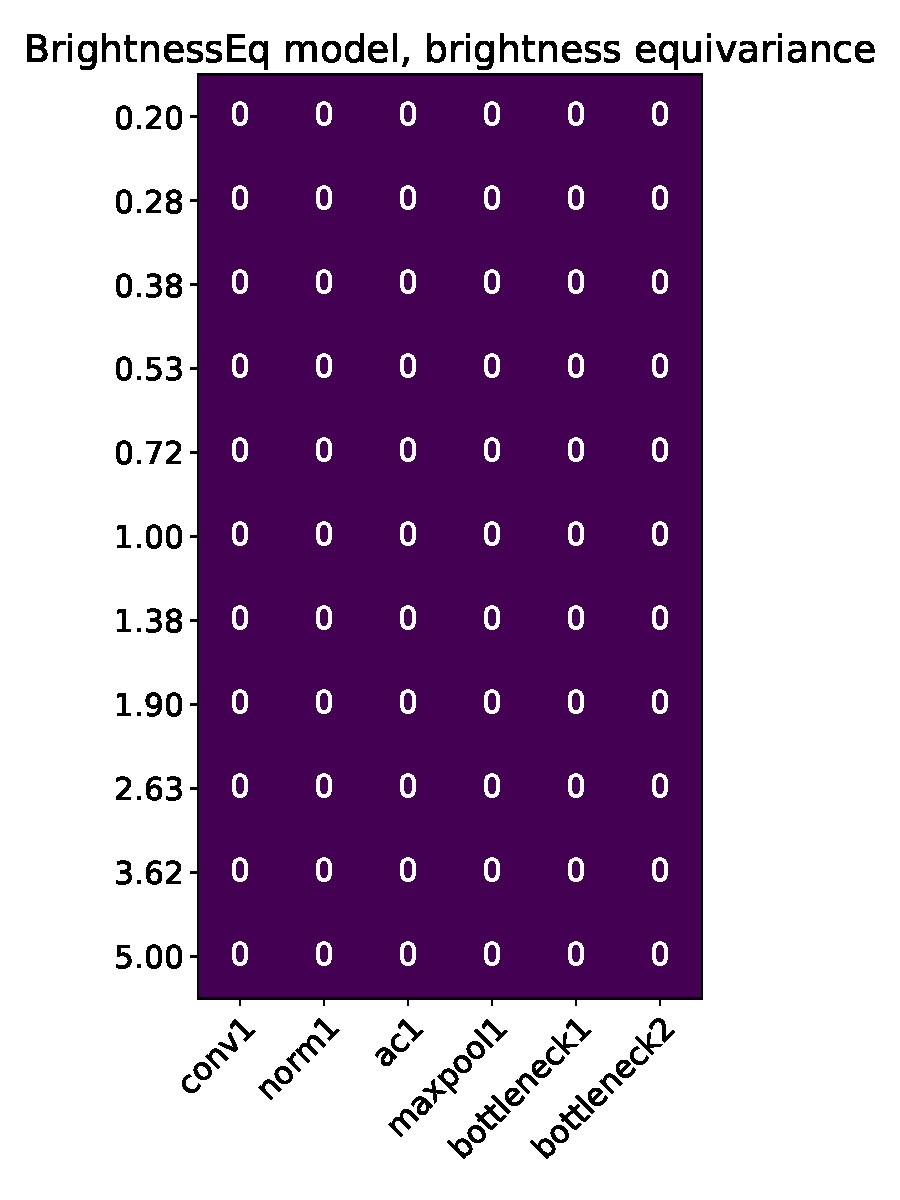
\includegraphics[width=\linewidth]{plots/plot7/BrightnessEq_brightness}
        \end{subfigure}
    \end{adjustwidth}
        \caption{Equivariance error to brightness transform of Plain and BrightnessEq
        model.}
        \label{fig:plot7brightness}
    \end{figure}

    \begin{figure}[h!]
    \begin{adjustwidth}{-11em}{-11em}
        \centering
        \begin{subfigure}{0.4\textwidth}
            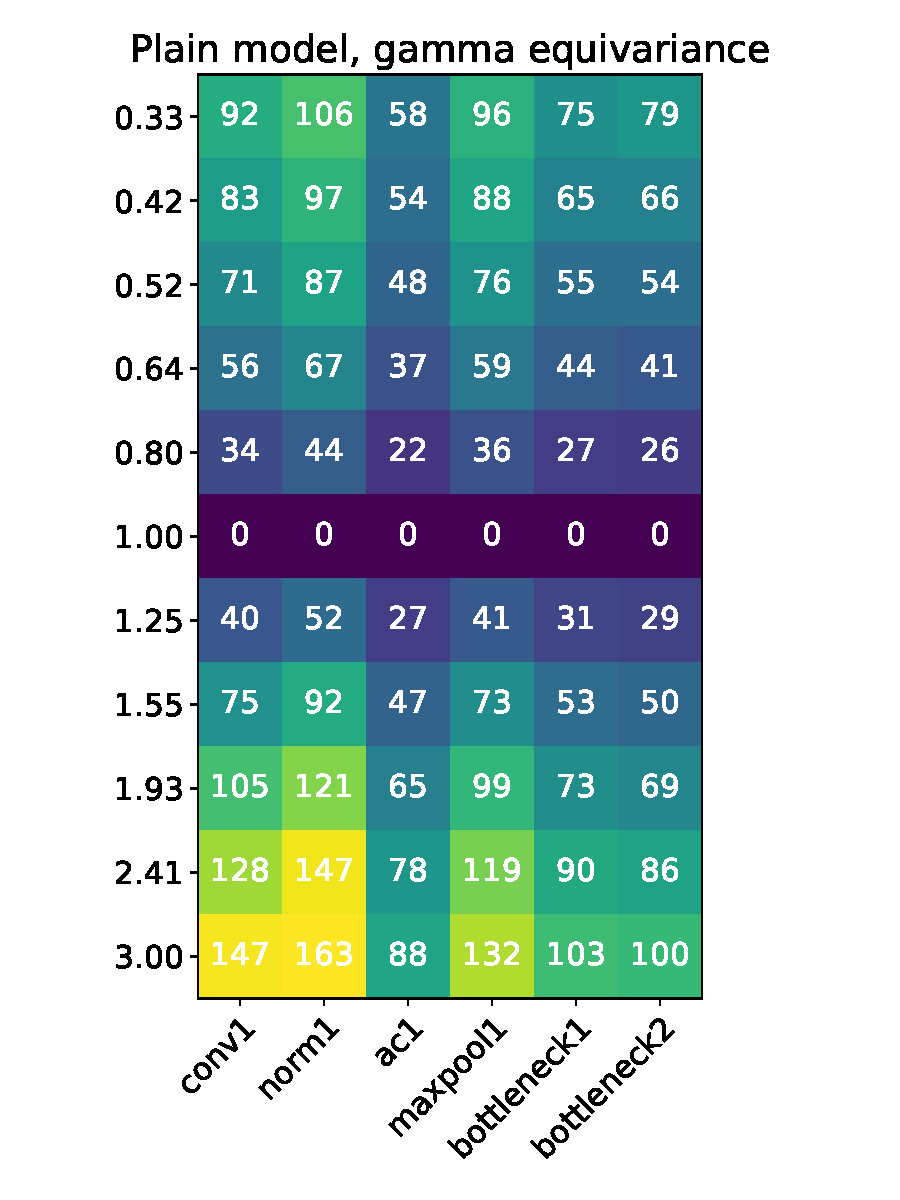
\includegraphics[width=\linewidth]{plots/plot7/plain_gamma}
        \end{subfigure}
        \begin{subfigure}{0.4\textwidth}
            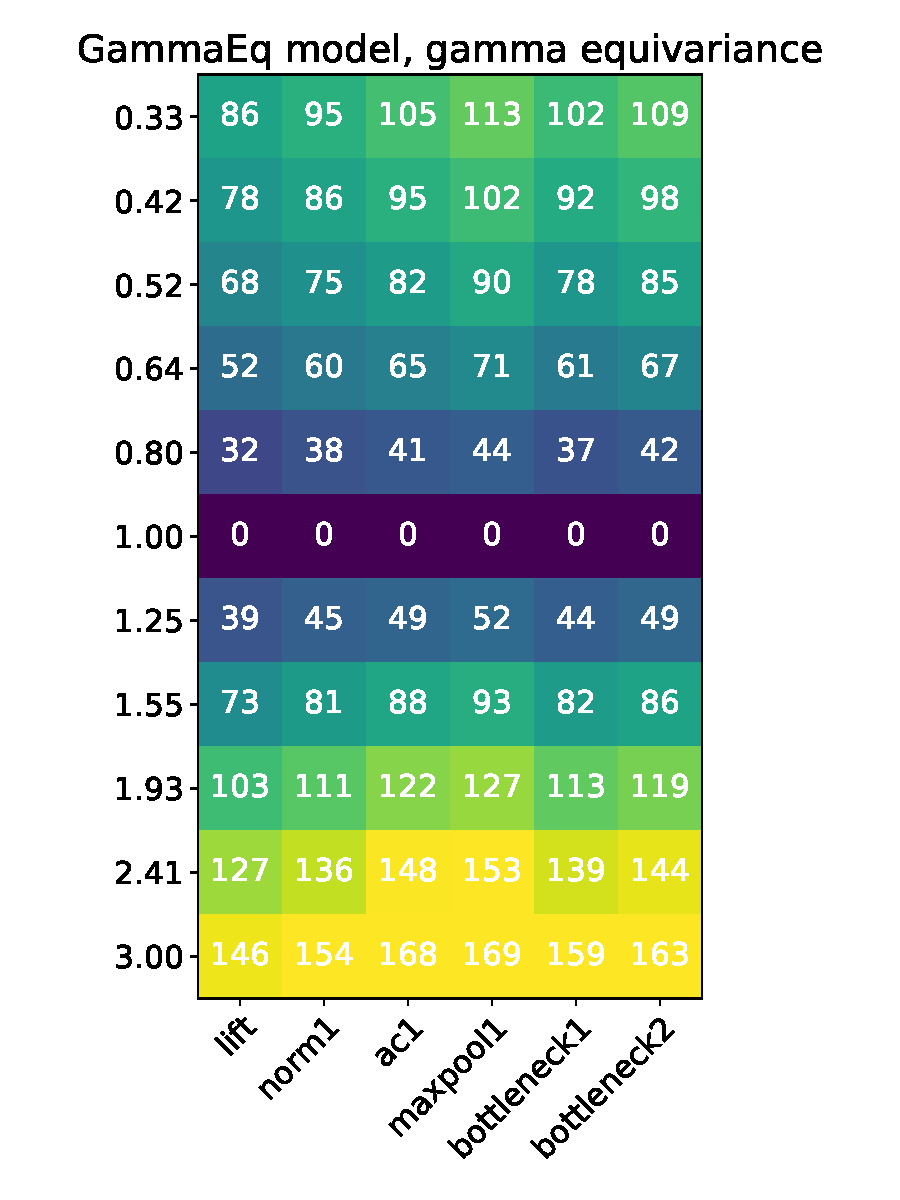
\includegraphics[width=\linewidth]{plots/plot7/GammaEq_gamma}
        \end{subfigure}
    \end{adjustwidth}
        \caption{Equivariance error to gamma transform of Plain and GammaEq
        model.}
        \label{fig:plot7gamma}
    \end{figure}

    \begin{figure}[h!]
    \begin{adjustwidth}{-11em}{-11em}
        \centering
        \begin{subfigure}{0.6\textwidth}
            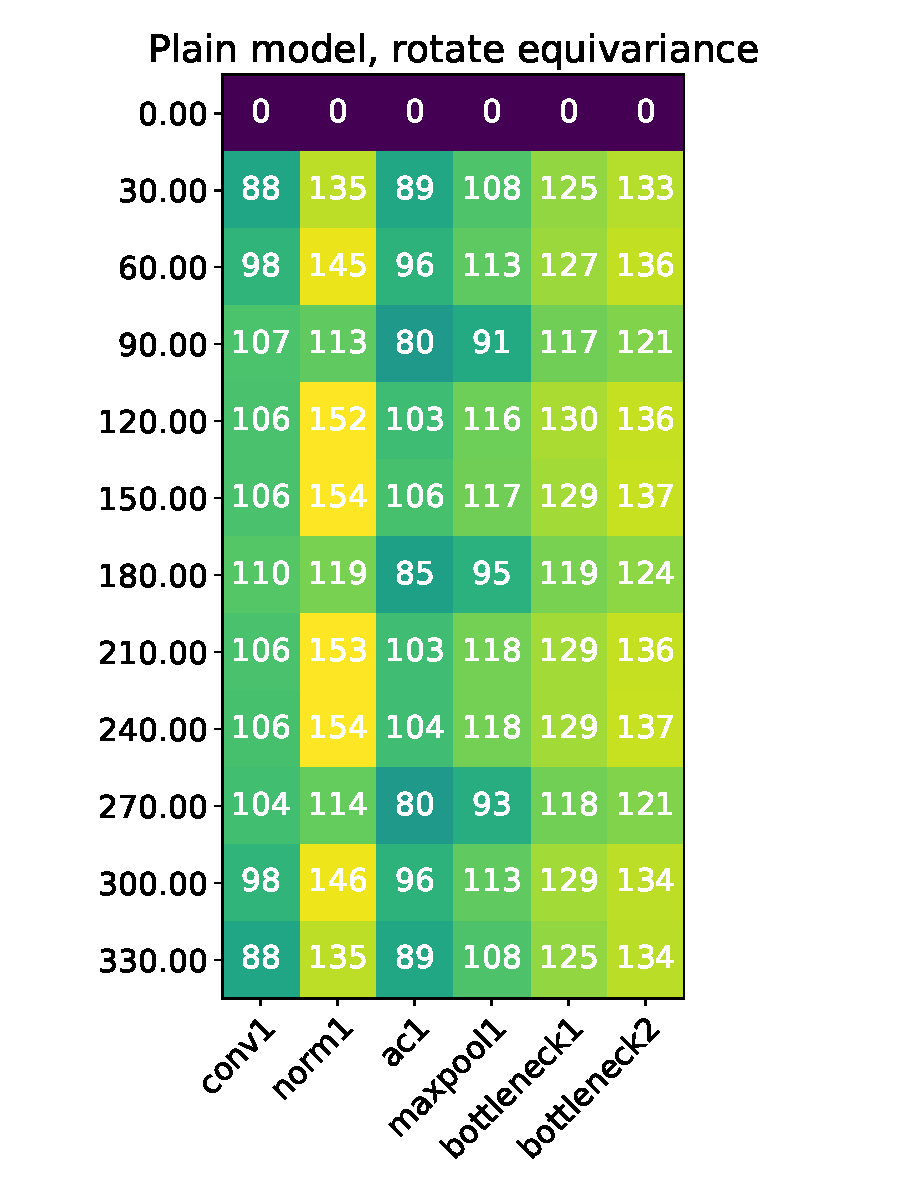
\includegraphics[width=\linewidth]{plots/plot7/plain_rotate}
        \end{subfigure}
        \begin{subfigure}{0.6\textwidth}
            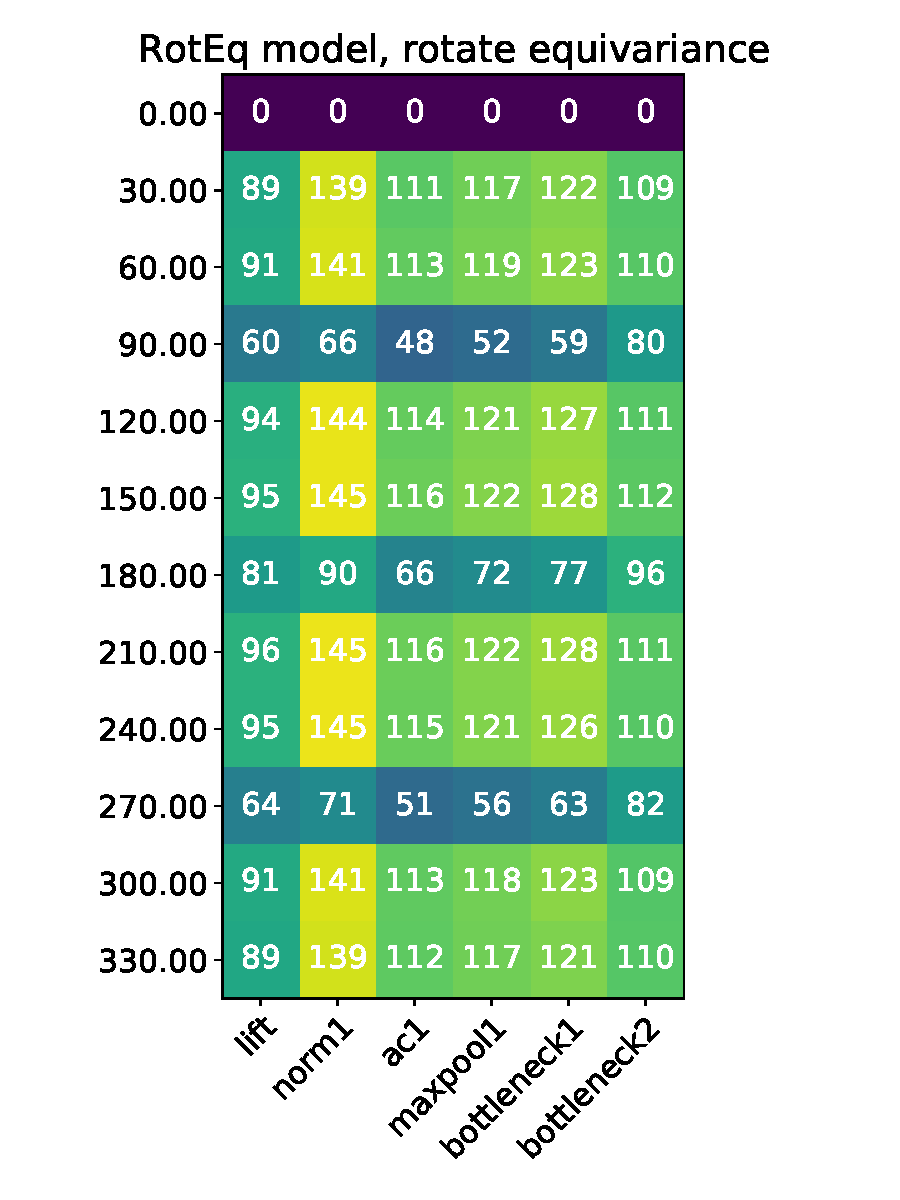
\includegraphics[width=\linewidth]{plots/plot7/RotEq_rotate}
        \end{subfigure}
    \end{adjustwidth}
        \caption{Equivariance error to rotations of Plain and RotEq
        model.}
        \label{fig:plot7rot}
    \end{figure}


    \begin{figure}[h!]
        \centering
        \begin{subfigure}{0.4\textwidth}
            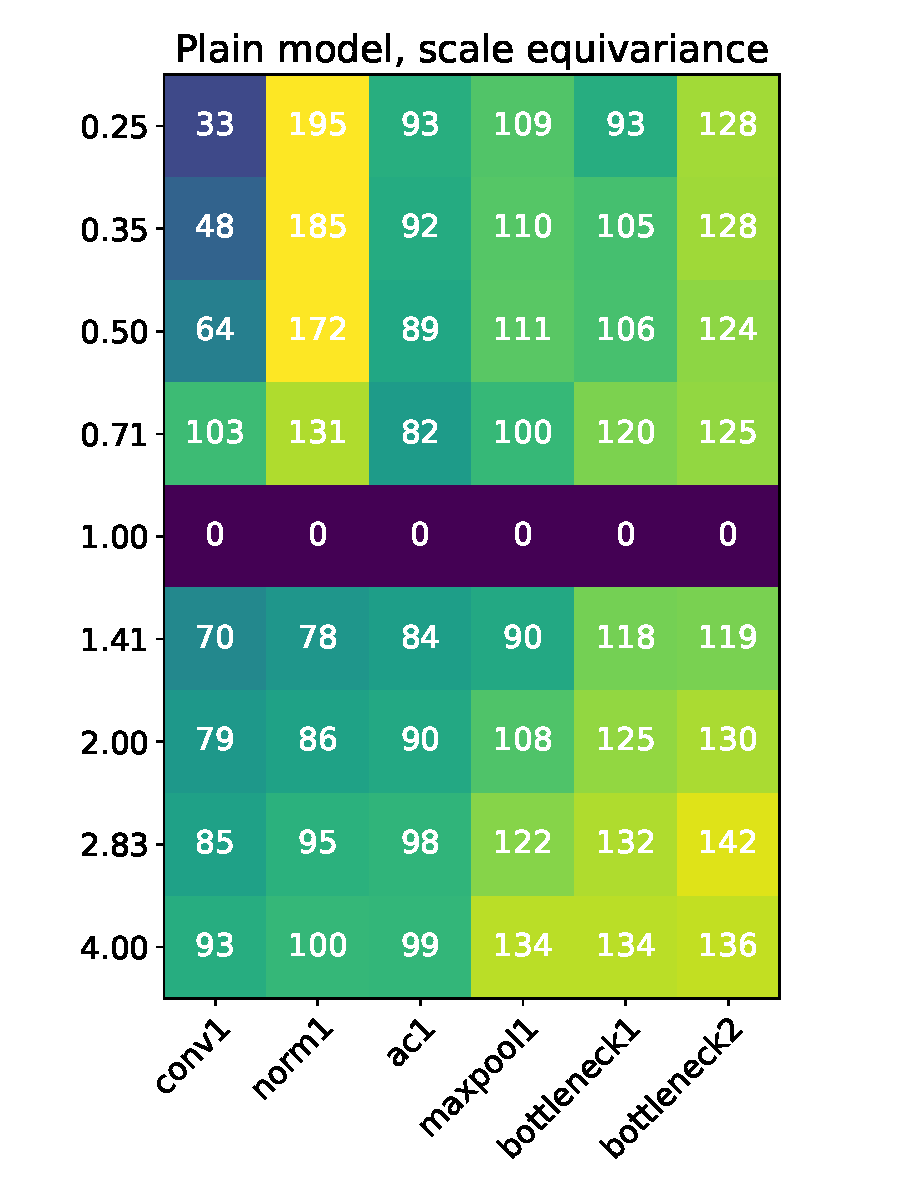
\includegraphics[width=\linewidth]{plots/plot7/plain_scale}
        \end{subfigure}
        \begin{subfigure}{0.4\textwidth}
            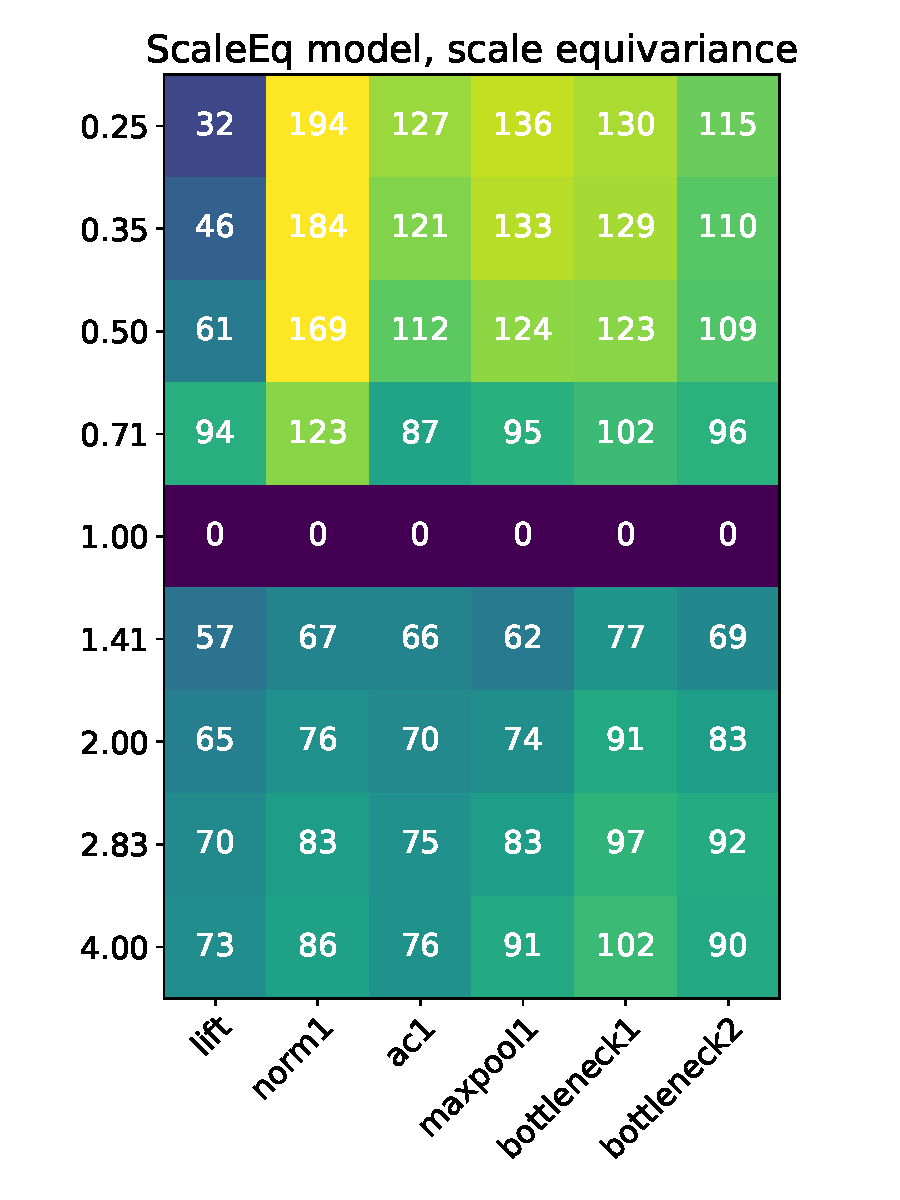
\includegraphics[width=\linewidth]{plots/plot7/ScaleEq_scale}
        \end{subfigure}
        \caption{Equivariance error to scaling of Plain and ScaleEq
        model.}
        \label{fig:plot7scale}
    \end{figure}


    \begin{figure}[h!]
        \centering
        \begin{subfigure}{0.4\textwidth}
            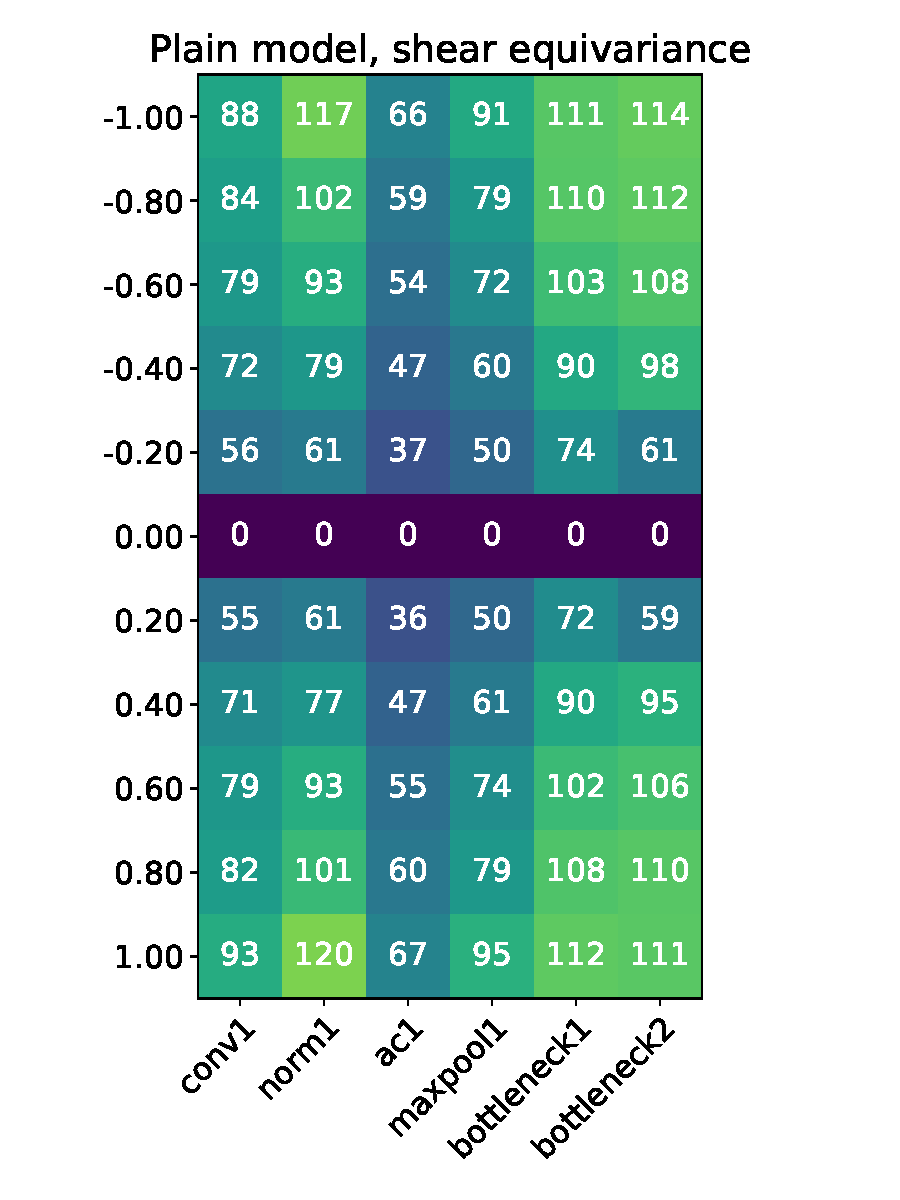
\includegraphics[width=\linewidth]{plots/plot7/plain_shear}
        \end{subfigure}
        \begin{subfigure}{0.4\textwidth}
            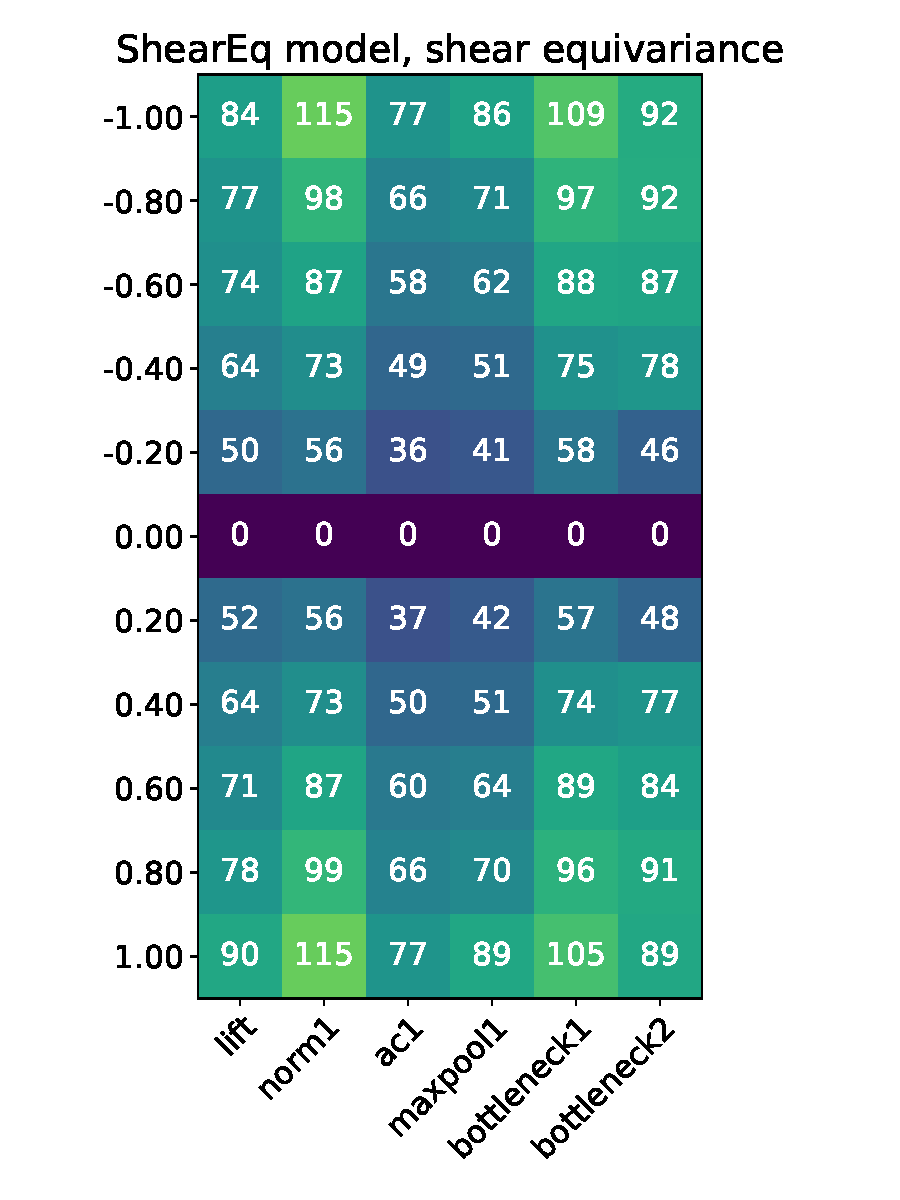
\includegraphics[width=\linewidth]{plots/plot7/SchearEq_shear}
        \end{subfigure}
        \caption{Equivariance error to shear transform of Plain and ShearEq
        model.}
        \label{fig:plot7shear}
    \end{figure}


    %%%%%%%% norms %%%%%%%%%%%%
    \subsubsection*{Gradient norms}
    \begin{figure}[h!]
        \centering
        \includegraphics[width=\textwidth]{plots/plot8/norms}
        \caption{Comparison of norms of gradients flowing through individual
            convolutional layers of PlainResNet and BResNet models.}
        \label{fig:plot8}
    \end{figure}


